% =====================================================================
%  PATRONUS -- Optimal VTOL take-off of a tilt-rotor UAV
%  Plain white 16:9 slides on the article class (no beamer).
%  All figures are TikZ / pgfplots (vector). Plot data come from the
%  solver (main_vtolto_optimizer, Hermite-Simpson stage) and are embedded
%  below as pgfplots tables.
%  Compile with pdflatex (twice, for the page count in the footer).
% =====================================================================
\documentclass[11pt]{article}

\usepackage[paperwidth=19.2cm, paperheight=10.8cm, left=0.9cm, right=0.9cm,
            top=0.7cm, bottom=0.95cm, footskip=0.5cm]{geometry}
\usepackage[utf8]{inputenc}
\usepackage[T1]{fontenc}
\usepackage{lmodern}
\usepackage[scaled=0.95]{helvet}
\renewcommand{\familydefault}{\sfdefault}
\usepackage{amsmath,amssymb}
\usepackage{booktabs}
\usepackage{xparse}
\usepackage{enumitem}
\usepackage{fancyhdr}
\usepackage{lastpage}
\usepackage{tikz}
\usetikzlibrary{arrows.meta,positioning,calc,shapes.geometric,fit,backgrounds}
\usepackage{pgfplots}
\pgfplotsset{compat=1.18}
\usepackage{pgfplotstable}
\usepgfplotslibrary{groupplots}
\usepackage[hidelinks]{hyperref}

% ---------------------------------------------------------------------
%  Plain white slide layout
% ---------------------------------------------------------------------
\definecolor{accent}{RGB}{20,60,110}
\definecolor{accent2}{RGB}{190,80,20}
\definecolor{muted}{RGB}{110,110,110}
\definecolor{good}{RGB}{30,120,60}

\setlength{\parindent}{0pt}
\setlength{\parskip}{3pt}
\raggedright

\setlist[itemize]{leftmargin=1.1em, itemsep=2pt, topsep=2pt, parsep=0pt, partopsep=0pt,
                  label={\color{accent}\small\textbullet}}
\setlist[itemize,2]{label={\color{muted}--}}
\setlist[enumerate]{leftmargin=1.4em, itemsep=3pt, topsep=2pt}

% Current section, shown in the footer
\newcommand{\cursec}{}
\renewcommand{\section}[1]{\gdef\cursec{#1}}

\fancypagestyle{slide}{%
  \fancyhf{}\renewcommand{\headrulewidth}{0pt}%
  \fancyfoot[L]{\scriptsize\color{muted}Optimal VTOL take-off of a tilt-rotor UAV}%
  \fancyfoot[R]{\scriptsize\color{muted}\cursec\quad\thepage/\pageref{LastPage}}}
\pagestyle{slide}

% One slide per page: \begin{frame}{Title} ... \end{frame}; [plain] = no title, no footer
\DeclareDocumentEnvironment{frame}{o g}
  {\clearpage
   \IfValueTF{#1}{\thispagestyle{empty}}{}%
   \IfValueT{#2}{{\Large\bfseries\color{accent}#2\par}\vspace{0.5mm}%
                 {\color{gray!35}\rule{\linewidth}{0.4pt}\par}\vspace{2.5mm}}}
  {\par\vfill\clearpage}% ship the page here, so the next \section only affects the next slide

% Side-by-side columns: \begin{columns}[T|c] \column{w} ... \column{w} ... \end{columns}
% (T = top-aligned, c = centred; each column is 3 mm narrower than w as gutter)
\newcommand{\colpos}{t}
\newcommand{\colstart}{}
\DeclareDocumentEnvironment{columns}{O{T}}
  {\par\noindent\def\colsep{}%
   \ifx T#1\def\colpos{t}\def\colstart{\vspace{0pt}}\else\def\colpos{c}\def\colstart{}\fi
   \ignorespaces}
  {\end{minipage}\par}
\newcommand{\column}[1]{\colsep
  \begin{minipage}[\colpos]{\dimexpr #1-3mm\relax}\colstart\def\colsep{\end{minipage}\hfill}}

% ---------------------------------------------------------------------
%  Plot styles
% ---------------------------------------------------------------------
\pgfplotsset{
  pres/.style={width=\linewidth, height=0.5\linewidth, grid=major, grid style={gray!25},
    tick label style={font=\scriptsize}, label style={font=\footnotesize},
    legend style={font=\scriptsize, draw=none, fill=white, fill opacity=0.85, text opacity=1},
    every axis plot/.append style={line width=1.1pt}, xmin=0, enlarge x limits=false},
  small/.style={pres, height=0.45\linewidth},
}
\newcommand{\cA}{accent}
\newcommand{\cB}{accent2}

% Tilt-rotor sketch (side view): #1 = tilt angle in degrees, #2 = body pitch
\newcommand{\aircraft}[2]{%
  \begin{scope}[rotate=#2]
    \fill[gray!35, draw=gray!70!black, rounded corners=2pt] (-1.6,-0.17) rectangle (1.6,0.17);
    \fill[gray!70] (0.55,0.15) rectangle (1.05,0.21);      % wing
    \fill[gray!70] (-1.35,0.15) rectangle (-0.85,0.21);    % tail
    \foreach \xp in {0.8,-1.1}{
      \begin{scope}[shift={(\xp,0.45)}, rotate=#1-90]
        \fill[gray!55, draw=gray!70!black] (-0.07,-0.25) rectangle (0.07,0.1);
        \draw[line width=1.6pt, gray!40!black] (-0.5,0.12) -- (0.5,0.12);
      \end{scope}}
  \end{scope}}

% ---- Solver data (main_vtolto_optimizer, Hermite-Simpson stage) ----
\pgfplotstableread{
 t x h vx vh theta q eps1 eps2 n1 n2 T1 T2 Ttot P E alpha V
 0.0000 0.0000 0.0000 -0.0000 0.0000 0.000 -0.0000 89.183 88.921 78.125 78.125 290.19 290.18 580.38 11.4068 -0.0000 -0.000 0.5000
 0.1164 0.0030 0.0860 0.0536 1.4619 0.092 0.0281 88.717 88.510 78.125 77.284 283.90 277.76 561.67 11.6987 0.0767 -71.008 1.5460
 0.2329 0.0128 0.3356 0.1147 2.8022 0.396 0.0648 88.338 88.231 78.125 75.086 278.96 257.21 536.16 11.5573 0.1533 -79.530 2.8487
 0.3493 0.0295 0.7331 0.1724 4.0018 0.982 0.1126 87.904 87.788 78.125 73.041 273.96 238.26 512.23 11.3776 0.2288 -82.097 4.0366
 0.4658 0.0526 1.2625 0.2222 5.0674 1.918 0.1686 87.268 87.066 77.762 71.578 266.29 223.63 489.91 11.1606 0.3030 -82.841 5.0968
 0.5822 0.0809 1.9073 0.2626 5.9796 3.227 0.2224 86.298 86.062 75.714 70.727 246.96 213.44 460.39 10.6088 0.3748 -82.538 6.0062
 0.6987 0.1134 2.6484 0.2946 6.7210 4.856 0.2634 84.988 84.833 73.075 70.386 224.70 207.09 431.79 9.9969 0.4426 -81.502 6.7461
 0.8151 0.1493 3.4668 0.3206 7.3129 6.707 0.2891 83.432 83.481 70.565 70.414 204.66 203.67 408.33 9.4855 0.5066 -79.995 7.3370
 0.9316 0.1879 4.3468 0.3416 7.7849 8.680 0.2998 81.749 82.108 68.374 70.670 187.85 202.21 390.06 9.0932 0.5677 -78.228 7.8084
 1.0480 0.2287 5.2762 0.3579 8.1633 10.677 0.2967 80.033 80.788 66.529 71.030 174.15 201.85 376.00 8.7998 0.6265 -76.364 8.1864
 1.1645 0.2711 6.2452 0.3695 8.4689 12.613 0.2819 78.353 79.554 65.012 71.392 163.14 201.91 365.05 8.5780 0.6836 -74.525 8.4917
 1.2809 0.3146 7.2463 0.3777 8.7170 14.416 0.2572 76.752 78.415 63.783 71.686 154.39 201.91 356.30 8.4033 0.7395 -72.796 8.7395
 1.3974 0.3590 8.2735 0.3844 8.9181 16.028 0.2247 75.259 77.366 62.800 71.867 147.50 201.51 349.02 8.2562 0.7943 -71.238 8.9404
 1.5138 0.4042 9.3217 0.3924 9.0793 17.402 0.1863 73.904 76.407 62.016 71.918 142.09 200.58 342.67 8.1225 0.8482 -69.885 9.1015
 1.6302 0.4505 10.3867 0.4047 9.2057 18.505 0.1437 72.727 75.560 61.387 71.836 137.83 199.08 336.90 7.9926 0.9012 -68.760 9.2281
 1.7467 0.4987 11.4644 0.4231 9.3005 19.313 0.0983 71.786 74.868 60.874 71.629 134.44 197.01 331.45 7.8597 0.9534 -67.878 9.3236
 1.8631 0.5493 12.5516 0.4485 9.3664 19.813 0.0515 71.132 74.374 60.442 71.301 131.69 194.40 326.09 7.7183 1.0046 -67.251 9.3904
 1.9796 0.6034 13.6447 0.4802 9.4046 20.000 0.0045 70.790 74.107 60.051 70.866 129.33 191.32 320.65 7.5645 1.0549 -66.887 9.4301
 2.0960 0.6614 14.7408 0.5173 9.4161 19.875 -0.0418 70.771 74.079 59.655 70.336 127.12 187.86 314.97 7.3948 1.1042 -66.793 9.4435
 2.2125 0.7240 15.8366 0.5582 9.4005 19.445 -0.0867 71.092 74.296 59.257 69.667 125.05 183.76 308.81 7.2015 1.1522 -66.966 9.4303
 2.3289 0.7915 16.9290 0.6013 9.3566 18.724 -0.1289 71.761 74.763 58.850 68.822 123.11 178.81 301.92 6.9775 1.1989 -67.403 9.3892
 2.4454 0.8640 18.0145 0.6441 9.2821 17.733 -0.1674 72.780 75.486 58.417 67.771 121.22 172.88 294.10 6.7175 1.2440 -68.091 9.3179
 2.5618 0.9414 19.0894 0.6840 9.1743 16.502 -0.2010 74.148 76.477 57.941 66.482 119.30 165.86 285.17 6.4170 1.2872 -69.013 9.2133
 2.6783 1.0231 20.1497 0.7178 9.0293 15.065 -0.2286 75.856 77.755 57.404 64.922 117.30 157.65 274.94 6.0724 1.3284 -70.147 9.0716
 2.7947 1.1082 21.1907 0.7422 8.8428 13.467 -0.2491 77.878 79.323 56.786 63.048 115.15 148.12 263.27 5.6817 1.3671 -71.462 8.8879
 2.9112 1.1954 22.2073 0.7542 8.6097 11.758 -0.2615 80.145 81.153 56.058 60.810 112.76 137.19 249.95 5.2437 1.4031 -72.920 8.6571
 3.0276 1.2833 23.1938 0.7521 8.3244 9.997 -0.2650 82.560 83.193 55.172 58.154 109.95 124.83 234.78 4.7587 1.4360 -74.468 8.3732
 3.1440 1.3700 24.1437 0.7353 7.9805 8.244 -0.2590 85.009 85.382 54.061 55.030 106.46 111.10 217.56 4.2294 1.4656 -76.037 8.0299
 3.2605 1.4540 25.0499 0.7050 7.5714 6.561 -0.2438 87.385 87.655 52.638 51.396 101.94 96.20 198.14 3.6627 1.4916 -77.546 7.6206
 3.3769 1.5338 25.9042 0.6636 7.0902 5.009 -0.2202 89.598 89.954 50.812 47.232 96.07 80.53 176.60 3.0721 1.5138 -78.901 7.1387
 3.4934 1.6082 26.6981 0.6146 6.5312 3.639 -0.1895 91.593 92.227 48.499 42.569 88.63 64.75 153.38 2.4802 1.5321 -79.995 6.5790
 3.6098 1.6768 27.4221 0.5620 5.8910 2.490 -0.1543 93.347 94.418 45.651 37.538 79.65 49.82 129.48 1.9186 1.5465 -80.715 5.9388
 3.7263 1.7391 28.0669 0.5097 5.1711 1.585 -0.1172 94.859 96.467 42.287 32.440 69.49 36.97 106.45 1.4226 1.5575 -80.939 5.2201
 3.8427 1.7956 28.6236 0.4605 4.3797 0.924 -0.0814 96.134 98.322 38.540 27.847 58.90 27.48 86.38 1.0231 1.5655 -80.527 4.4321
 3.9592 1.8465 29.0848 0.4149 3.5336 0.489 -0.0499 97.168 99.954 34.723 24.745 49.09 22.68 71.77 0.7416 1.5712 -79.262 3.5928
 4.0756 1.8923 29.4455 0.3700 2.6614 0.243 -0.0254 97.933 101.344 31.445 24.879 41.68 25.06 66.74 0.6048 1.5755 -76.699 2.7331
 4.1921 1.9324 29.7057 0.3162 1.8176 0.127 -0.0114 98.380 102.343 29.829 29.719 39.12 38.96 78.08 0.6785 1.5796 -71.903 1.9115
 4.3085 1.9651 29.8725 0.2415 1.0689 0.067 -0.0076 98.391 102.369 32.127 35.542 47.29 58.24 105.53 0.9793 1.5848 -62.519 1.2045
 4.4250 1.9876 29.9614 0.1420 0.4908 0.024 -0.0048 97.601 100.161 37.949 41.364 67.72 80.61 148.34 1.5380 1.5930 -43.351 0.7149
 4.5414 1.9982 29.9951 0.0444 0.1261 0.004 -0.0016 94.991 95.240 43.771 47.186 91.10 105.86 196.96 2.2638 1.6054 -14.096 0.5175
 4.6579 2.0000 30.0000 0.0000 0.0000 0.000 -0.0000 89.996 90.000 49.594 53.009 117.09 133.74 250.84 3.2162 1.6233 -0.000 0.5000
}\tabres

\pgfplotstableread{
 t x h vh theta eps1 n1 n2 E
 0.0000 0.0000 0.0000 0.0000 0.000 90.000 49.565 52.978 0.0000
 0.4000 0.0012 0.0181 0.1327 0.000 89.768 51.253 54.712 0.0769
 0.8000 0.0091 0.1358 0.4875 0.000 89.636 52.688 56.193 0.1626
 1.2000 0.0286 0.4296 1.0036 0.000 89.577 53.856 57.418 0.2560
 1.6000 0.0635 0.9528 1.6257 0.000 89.551 54.769 58.403 0.3564
 2.0000 0.1158 1.7376 2.3040 0.000 89.571 55.497 59.237 0.4633
 2.4000 0.1865 2.7975 2.9943 0.000 89.625 56.076 59.951 0.5759
 2.8000 0.2753 4.1294 3.6578 0.000 89.705 56.509 60.541 0.6934
 3.2000 0.3811 5.7158 4.2615 0.000 89.805 56.781 60.978 0.8148
 3.6000 0.5018 7.5269 4.7776 0.000 89.922 56.864 61.220 0.9386
 4.0000 0.6349 9.5232 5.1840 0.000 90.050 56.733 61.224 1.0632
 4.4000 0.7772 11.6573 5.4642 0.000 90.186 56.363 60.951 1.1869
 4.8000 0.9251 13.8762 5.6070 0.000 90.326 55.743 60.380 1.3079
 5.2000 1.0749 16.1238 5.6070 0.000 90.467 54.879 59.507 1.4244
 5.6000 1.2228 18.3427 5.4642 0.000 90.604 53.795 58.357 1.5348
 6.0000 1.3651 20.4768 5.1840 0.000 90.734 52.536 56.978 1.6382
 6.4000 1.4982 22.4731 4.7776 0.000 90.851 51.172 55.449 1.7339
 6.8000 1.6189 24.2842 4.2615 0.000 90.946 49.793 53.876 1.8217
 7.2000 1.7247 25.8706 3.6578 0.000 91.009 48.504 52.383 1.9021
 7.6000 1.8135 27.2025 2.9943 0.000 91.028 47.422 51.109 1.9759
 8.0000 1.8842 28.2624 2.3040 0.000 90.992 46.655 50.182 2.0445
 8.4000 1.9365 29.0472 1.6257 0.000 90.896 46.293 49.709 2.1094
 8.8000 1.9714 29.5704 1.0036 0.000 90.746 46.384 49.746 2.1724
 9.2000 1.9909 29.8642 0.4875 0.000 90.519 46.926 50.272 2.2356
 9.6000 1.9988 29.9819 0.1327 0.000 90.265 47.963 51.331 2.3009
 10.0000 2.0000 30.0000 0.0000 0.000 90.000 49.565 52.978 2.3703
}\tabguess

\pgfplotstableread{
 k obj infpr infdu
 0 2.370552e+00 1.000e-02 4.073e-01
 1 2.372237e+00 2.263e-02 2.953e+00
 2 2.369886e+00 2.404e-02 2.464e+02
 3 2.365533e+00 2.402e-02 2.934e+02
 4 2.355840e+00 3.097e-02 3.364e+02
 5 2.323656e+00 1.205e-01 2.849e+02
 6 2.319151e+00 1.184e-01 3.477e+02
 7 2.309856e+00 9.324e-02 4.497e+01
 8 2.576669e+00 9.201e-03 1.488e+02
 9 2.703277e+00 5.373e-03 8.237e+02
 10 2.786509e+00 1.227e-03 7.406e-02
 11 2.209389e+00 5.943e-02 1.846e+03
 12 1.969533e+00 2.797e-02 6.579e+02
 13 1.750765e+00 6.063e-02 1.455e+02
 14 1.709291e+00 2.390e-02 2.460e-02
 15 1.640978e+00 4.175e-02 3.185e+01
 16 1.633593e+00 1.964e-02 3.567e-03
 17 1.632474e+00 5.499e-03 6.396e-04
 18 1.633094e+00 6.201e-05 5.543e-06
 19 1.628466e+00 5.124e-03 1.970e+00
 20 1.628388e+00 1.315e-03 4.557e-01
 21 1.628413e+00 3.369e-04 1.016e-04
 22 1.628416e+00 4.591e-05 1.236e-05
 23 1.628419e+00 7.016e-07 1.531e-07
 24 1.628390e+00 1.887e-05 2.752e-02
 25 1.628381e+00 6.515e-06 5.816e-03
 26 1.628382e+00 2.145e-07 2.241e-08
 27 1.628382e+00 5.743e-08 5.886e-09
 28 1.628382e+00 4.905e-09 4.242e-10
}\tabconvA

\pgfplotstableread{
 k obj infpr infdu
 0 1.628382e+00 1.000e-02 3.486e-01
 1 1.630705e+00 7.840e-03 1.118e+00
 2 1.648579e+00 6.208e-02 9.224e+01
 3 1.680167e+00 4.529e-02 1.923e+01
 4 1.797418e+00 1.529e-01 2.385e+01
 5 2.135829e+00 1.359e-01 7.959e+01
 6 2.751213e+00 1.237e-01 1.287e+02
 7 2.969118e+00 4.662e-02 3.434e+02
 8 3.081725e+00 1.187e-02 4.597e+02
 9 3.127117e+00 3.121e-04 1.384e+01
 10 3.128158e+00 1.805e-07 6.521e-02
 11 2.360804e+00 7.368e-02 2.056e+03
 12 2.113274e+00 3.310e-02 8.039e+02
 13 1.842422e+00 5.012e-02 2.565e+02
 14 1.760730e+00 2.641e-02 4.045e-02
 15 1.738087e+00 7.220e-03 3.409e-03
 16 1.648746e+00 3.818e-02 3.121e+01
 17 1.636692e+00 1.810e-02 3.626e-03
 18 1.634301e+00 5.734e-03 4.205e-04
 19 1.634980e+00 5.448e-05 3.311e-06
 20 1.628008e+00 7.087e-03 2.088e+00
 21 1.627841e+00 2.002e-03 5.316e-01
 22 1.627835e+00 4.763e-04 1.180e-04
 23 1.627836e+00 5.896e-05 1.627e-05
 24 1.627840e+00 1.113e-06 2.428e-07
 25 1.627791e+00 3.584e-05 2.491e-02
 26 1.627777e+00 1.446e-05 2.507e-03
 27 1.627777e+00 2.736e-07 2.797e-08
 28 1.627777e+00 4.276e-09 4.018e-10
}\tabconvB

% n1 <= 78.125  sum lambda = 0.06342, active 8/81
\pgfplotstableread{
 t value lam
 0.0000 78.125 5.53312e-03
 0.0582 78.125 1.85505e-02
 0.1164 78.125 7.81757e-03
 0.1747 78.125 1.29095e-02
 0.2329 78.125 5.13848e-03
 0.2911 78.125 7.89560e-03
 0.3493 78.125 2.79974e-03
 0.4076 78.125 2.77886e-03
 0.4658 77.762 5.37375e-07
 0.5240 76.945 1.62957e-07
 0.5822 75.714 7.82161e-08
 0.6405 74.405 4.95861e-08
 0.6987 73.075 3.56617e-08
 0.7569 71.776 2.76671e-08
 0.8151 70.565 2.26638e-08
 0.8733 69.414 1.91784e-08
 0.9316 68.374 1.67225e-08
 0.9898 67.397 1.48376e-08
 1.0480 66.529 1.34199e-08
 1.1062 65.721 1.22697e-08
 1.1645 65.012 1.13705e-08
 1.2227 64.355 1.06155e-08
 1.2809 63.783 1.00108e-08
 1.3391 63.257 9.49110e-09
 1.3974 62.8 9.06731e-09
 1.4556 62.38 8.69674e-09
 1.5138 62.016 8.38947e-09
 1.5720 61.68 8.11660e-09
 1.6302 61.387 7.88635e-09
 1.6885 61.114 7.67888e-09
 1.7467 60.874 7.50015e-09
 1.8049 60.648 7.33630e-09
 1.8631 60.442 7.19017e-09
 1.9214 60.244 7.05227e-09
 1.9796 60.051 6.92010e-09
 2.0378 59.854 6.78812e-09
 2.0960 59.655 6.65719e-09
 2.1543 59.457 6.52846e-09
 2.2125 59.257 6.40155e-09
 2.2707 59.056 6.27569e-09
 2.3289 58.85 6.14914e-09
 2.3871 58.639 6.02172e-09
 2.4454 58.417 5.89048e-09
 2.5036 58.187 5.75655e-09
 2.5618 57.941 5.61606e-09
 2.6200 57.683 5.47155e-09
 2.6783 57.404 5.31825e-09
 2.7365 57.109 5.15988e-09
 2.7947 56.786 4.99006e-09
 2.8529 56.442 4.81351e-09
 2.9112 56.058 4.62112e-09
 2.9694 55.644 4.41933e-09
 3.0276 55.172 4.19537e-09
 3.0858 54.658 3.95859e-09
 3.1440 54.061 3.69214e-09
 3.2023 53.405 3.40945e-09
 3.2605 52.638 3.08988e-09
 3.3187 51.796 2.75151e-09
 3.3769 50.812 2.37079e-09
 3.4352 49.737 1.96972e-09
 3.4934 48.499 1.52296e-09
 3.5516 47.16 1.05413e-09
 3.6098 45.651 5.37243e-10
 3.6681 44.044 0.00000e+00
 3.7263 42.287 0.00000e+00
 3.7845 40.455 0.00000e+00
 3.8427 38.54 0.00000e+00
 3.9010 36.603 0.00000e+00
 3.9592 34.723 0.00000e+00
 4.0174 32.923 0.00000e+00
 4.0756 31.445 0.00000e+00
 4.1338 30.231 0.00000e+00
 4.1921 29.829 0.00000e+00
 4.2503 30.052 0.00000e+00
 4.3085 32.127 0.00000e+00
 4.3667 35.038 0.00000e+00
 4.4250 37.949 0.00000e+00
 4.4832 40.86 0.00000e+00
 4.5414 43.771 0.00000e+00
 4.5996 46.682 8.89419e-10
 4.6579 49.594 1.91713e-09
}\tablamA

% x(tf) <= 2  sum lambda = 0.05782, active 1/1
\pgfplotstableread{
 t value lam
 4.6579 -3.3338e-08 5.78216e-02
}\tablamB

% dn2/dt <= 50  sum lambda = 0.02323, active 9/80
\pgfplotstableread{
 t value lam
 0.0291 -0.013944 2.50541e-09
 0.0873 -14.423 1.94488e-09
 0.1456 -17.971 1.84333e-09
 0.2038 -19.793 1.79522e-09
 0.2620 -18.873 1.81921e-09
 0.3202 -16.25 1.89121e-09
 0.3785 -14.288 1.94894e-09
 0.4367 -10.83 2.05975e-09
 0.4949 -8.8841 2.12780e-09
 0.5531 -5.7286 2.24829e-09
 0.6113 -4.1561 2.31357e-09
 0.6696 -1.707 2.42315e-09
 0.7278 -0.59033 2.47664e-09
 0.7860 1.0692 2.56064e-09
 0.8442 1.7406 2.59626e-09
 0.9025 2.6622 2.64681e-09
 0.9607 2.9388 2.66237e-09
 1.0189 3.2372 2.67935e-09
 1.0771 3.1988 2.67716e-09
 1.1354 3.0252 2.66726e-09
 1.1936 2.7646 2.65255e-09
 1.2518 2.2786 2.62553e-09
 1.3100 1.8867 2.60414e-09
 1.3682 1.2337 2.56928e-09
 1.4265 0.78757 2.54598e-09
 1.4847 0.083558 2.51007e-09
 1.5429 -0.36073 2.48793e-09
 1.6011 -1.0427 2.45469e-09
 1.6594 -1.4609 2.43474e-09
 1.7176 -2.1069 2.40456e-09
 1.7758 -2.5067 2.38625e-09
 1.8340 -3.1169 2.35883e-09
 1.8923 -3.4905 2.34235e-09
 1.9505 -3.9928 2.32057e-09
 2.0087 -4.26 2.30914e-09
 2.0669 -4.8437 2.28456e-09
 2.1251 -5.3139 2.26514e-09
 2.1834 -6.1616 2.23095e-09
 2.2416 -6.7466 2.20795e-09
 2.2998 -7.7668 2.16896e-09
 2.3580 -8.4441 2.14382e-09
 2.4163 -9.6204 2.10152e-09
 2.4745 -10.392 2.07467e-09
 2.5327 -11.74 2.02938e-09
 2.5909 -12.621 2.00083e-09
 2.6492 -14.175 1.95237e-09
 2.7074 -15.19 1.92198e-09
 2.7656 -16.998 1.87010e-09
 2.8238 -18.174 1.83785e-09
 2.8820 -20.269 1.78306e-09
 2.9403 -21.612 1.74960e-09
 2.9985 -23.998 1.69320e-09
 3.0567 -25.502 1.65947e-09
 3.1149 -28.153 1.60318e-09
 3.1732 -29.79 1.57029e-09
 3.2314 -32.632 1.51628e-09
 3.2896 -34.333 1.48569e-09
 3.3478 -37.185 1.43709e-09
 3.4061 -38.804 1.41089e-09
 3.4643 -41.278 1.37265e-09
 3.5225 -42.526 1.35413e-09
 3.5807 -43.89 1.33447e-09
 3.6389 -44.266 1.32914e-09
 3.6972 -43.295 1.34298e-09
 3.7554 -42.018 1.36162e-09
 3.8136 -36.854 1.44256e-09
 3.8718 -32.763 1.51387e-09
 3.9301 -20.518 1.77675e-09
 3.9883 -11.575 2.03482e-09
 4.0465 13.87 3.46787e-09
 4.1047 33.14 7.43137e-09
 4.1630 49.999 1.85281e-04
 4.2212 50 3.78676e-04
 4.2794 50 9.13843e-04
 4.3376 50 1.26637e-03
 4.3958 50 2.16303e-03
 4.4541 50 2.71954e-03
 4.5123 50 4.06270e-03
 4.5705 50 4.85921e-03
 4.6287 50 6.68288e-03
}\tablamC

% dn1/dt <= 50  sum lambda = 0.006643, active 6/80
\pgfplotstableread{
 t value lam
 0.0291 0.00042644 2.50590e-09
 0.0873 -0.00024886 2.50587e-09
 0.1456 0.00016965 2.50589e-09
 0.2038 -0.0003939 2.50586e-09
 0.2620 0.0002285 2.50589e-09
 0.3202 -0.00077513 2.50584e-09
 0.3785 -9.0392e-06 2.50588e-09
 0.4367 -6.2255 2.22842e-09
 0.4949 -14.044 1.95637e-09
 0.5531 -21.142 1.76119e-09
 0.6113 -22.482 1.72862e-09
 0.6696 -22.845 1.72001e-09
 0.7278 -22.304 1.73286e-09
 0.7860 -20.801 1.76966e-09
 0.8442 -19.776 1.79566e-09
 0.9025 -17.865 1.84621e-09
 0.9607 -16.776 1.87633e-09
 1.0189 -14.901 1.93052e-09
 1.0771 -13.88 1.96138e-09
 1.1354 -12.184 2.01488e-09
 1.1936 -11.279 2.04463e-09
 1.2518 -9.8151 2.09468e-09
 1.3100 -9.0478 2.12190e-09
 1.3682 -7.8363 2.16635e-09
 1.4265 -7.2147 2.18989e-09
 1.4847 -6.2547 2.22726e-09
 1.5429 -5.7729 2.24650e-09
 1.6011 -5.038 2.27650e-09
 1.6594 -4.6756 2.29159e-09
 1.7176 -4.1348 2.31448e-09
 1.7758 -3.88 2.32542e-09
 1.8340 -3.5344 2.34043e-09
 1.8923 -3.401 2.34628e-09
 1.9505 -3.3206 2.34982e-09
 2.0087 -3.3769 2.34734e-09
 2.0669 -3.411 2.34584e-09
 2.1251 -3.4147 2.34568e-09
 2.1834 -3.4263 2.34517e-09
 2.2416 -3.4579 2.34379e-09
 2.2998 -3.5379 2.34028e-09
 2.3580 -3.6256 2.33646e-09
 2.4163 -3.8018 2.32880e-09
 2.4745 -3.9512 2.32236e-09
 2.5327 -4.2242 2.31066e-09
 2.5909 -4.431 2.30189e-09
 2.6492 -4.7975 2.28649e-09
 2.7074 -5.0629 2.27547e-09
 2.7656 -5.5516 2.25545e-09
 2.8238 -5.9084 2.24105e-09
 2.8820 -6.5996 2.21368e-09
 2.9403 -7.1057 2.19407e-09
 2.9985 -8.1089 2.15619e-09
 3.0567 -8.8312 2.12972e-09
 3.1149 -10.257 2.07932e-09
 3.1732 -11.253 2.04552e-09
 3.2314 -13.177 1.98320e-09
 3.2896 -14.471 1.94340e-09
 3.3478 -16.896 1.87295e-09
 3.4061 -18.457 1.83025e-09
 3.4643 -21.27 1.75801e-09
 3.5225 -22.99 1.71658e-09
 3.5807 -25.923 1.65027e-09
 3.6389 -27.597 1.61466e-09
 3.6972 -30.173 1.56279e-09
 3.7554 -31.467 1.53797e-09
 3.8136 -32.895 1.51146e-09
 3.8718 -33.278 1.50451e-09
 3.9301 -32.283 1.52271e-09
 3.9883 -30.915 1.54846e-09
 4.0465 -25.393 1.66187e-09
 4.1047 -20.843 1.76862e-09
 4.1630 -6.9018 2.20193e-09
 4.2212 3.8267 2.71356e-09
 4.2794 35.637 8.72355e-09
 4.3376 49.998 5.02458e-05
 4.3958 50 3.97843e-04
 4.4541 50 6.40773e-04
 4.5123 50 1.27329e-03
 4.5705 50 1.67092e-03
 4.6287 50 2.61025e-03
}\tablamD

% theta <= 0.349066  sum lambda = 0.003968, active 1/39
\pgfplotstableread{
 t value lam
 0.1164 0.0016057 6.60477e-11
 0.2329 0.0069067 2.84197e-10
 0.3493 0.017139 7.06661e-10
 0.4658 0.033469 1.38944e-09
 0.5822 0.056319 2.37842e-09
 0.6987 0.084745 3.70407e-09
 0.8151 0.11707 5.42533e-09
 0.9316 0.15149 7.67709e-09
 1.0480 0.18634 1.07196e-08
 1.1645 0.22014 1.50341e-08
 1.2809 0.25161 2.15423e-08
 1.3974 0.27974 3.21626e-08
 1.5138 0.30373 5.14297e-08
 1.6302 0.32297 9.23082e-08
 1.7467 0.33708 2.05418e-07
 1.8631 0.34581 7.65579e-07
 1.9796 0.34907 3.96475e-03
 2.0960 0.34688 1.14287e-06
 2.2125 0.33938 2.55024e-07
 2.3289 0.3268 1.08826e-07
 2.4454 0.30951 5.95418e-08
 2.5618 0.28801 3.71075e-08
 2.6783 0.26293 2.49978e-08
 2.7947 0.23504 1.76862e-08
 2.9112 0.20522 1.29001e-08
 3.0276 0.17448 9.56688e-09
 3.1440 0.14388 7.12923e-09
 3.2605 0.11451 5.27824e-09
 3.3769 0.087424 3.83657e-09
 3.4934 0.063513 2.70186e-09
 3.6098 0.043464 1.81589e-09
 3.7263 0.027659 1.14485e-09
 3.8427 0.016128 6.64811e-10
 3.9592 0.0085406 3.51501e-10
 4.0756 0.0042393 1.74397e-10
 4.1921 0.0022132 9.10363e-11
 4.3085 0.0011648 4.79101e-11
 4.4250 0.00042742 1.75806e-11
 4.5414 6.373e-05 2.62134e-12
}\tablamE

% phi2 <= 90 deg  sum lambda = 0.003615, active 1/41
\pgfplotstableread{
 t value lam
 0.0000 -0.011991 2.09034e-07
 0.1164 -0.80553 3.11087e-09
 0.2329 -0.90332 2.77407e-09
 0.3493 -0.93677 2.67503e-09
 0.4658 -0.95306 2.62929e-09
 0.5822 -0.96084 2.60800e-09
 0.6987 -0.96298 2.60221e-09
 0.8151 -0.96127 2.60686e-09
 0.9316 -0.95688 2.61879e-09
 1.0480 -0.95084 2.63543e-09
 1.1645 -0.94412 2.65421e-09
 1.2809 -0.93758 2.67272e-09
 1.3974 -0.93191 2.68896e-09
 1.5138 -0.92753 2.70166e-09
 1.6302 -0.92445 2.71067e-09
 1.7467 -0.92234 2.71689e-09
 1.8631 -0.92085 2.72128e-09
 1.9796 -0.91978 2.72444e-09
 2.0960 -0.91904 2.72662e-09
 2.2125 -0.91856 2.72807e-09
 2.3289 -0.91822 2.72907e-09
 2.4454 -0.91783 2.73021e-09
 2.5618 -0.91706 2.73251e-09
 2.6783 -0.91546 2.73728e-09
 2.7947 -0.91266 2.74568e-09
 2.9112 -0.90853 2.75817e-09
 3.0276 -0.90305 2.77490e-09
 3.1440 -0.89617 2.79621e-09
 3.2605 -0.88768 2.82294e-09
 3.3769 -0.87718 2.85673e-09
 3.4934 -0.86409 2.90003e-09
 3.6098 -0.84774 2.95595e-09
 3.7263 -0.82747 3.02838e-09
 3.8427 -0.80228 3.12343e-09
 3.9592 -0.77009 3.25402e-09
 4.0756 -0.72617 3.45081e-09
 4.1921 -0.66178 3.78659e-09
 4.3085 -0.55722 4.49711e-09
 4.4250 -0.36877 6.79521e-09
 4.5414 -0.098402 2.54660e-08
 4.6579 -6.8094e-07 3.61513e-03
}\tablamF



% =====================================================================
\begin{document}

\begin{frame}[plain]
  \vspace*{9mm}
  {\LARGE\bfseries\color{accent} Optimal VTOL take-off of a tilt-rotor UAV\par}
  \vspace{2mm}
  {\large Direct collocation, nonlinear programming\\and what the multipliers tell us\par}
  \vspace{6mm}
  {\normalsize Álvaro Martínez Blanco\par}
  {\small\color{muted} PhD programme -- Universidad de Sevilla \quad\textbullet\quad \today\par}
  \vfill
  \hfill
  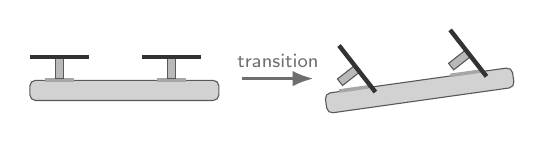
\begin{tikzpicture}[scale=0.75]
    \aircraft{90}{0}
    \begin{scope}[xshift=5cm] \aircraft{30}{8} \end{scope}
    \draw[-{Latex}, muted, line width=1pt] (2.0,0.2) -- node[above, font=\scriptsize]{transition} (3.2,0.2);
  \end{tikzpicture}
\end{frame}

\begin{frame}{Outline}
  \vspace{4mm}
  \begin{enumerate}\large
    \item[\color{accent}1.] Motivation \hfill{\small\color{muted} why a tilt-rotor, why take-off, why optimise}
    \item[\color{accent}2.] Models \hfill{\small\color{muted} dynamics, aero, rotors, nacelle, downwash, battery}
    \item[\color{accent}3.] Problem formulation \hfill{\small\color{muted} direct method, transcription, CasADi, IPOPT}
    \item[\color{accent}4.] Initial guess \hfill{\small\color{muted} differential flatness, what to expect}
    \item[\color{accent}5.] Results \hfill{\small\color{muted} trajectory, controls, multipliers, animation}
    \item[\color{accent}6.] Future work \hfill{\small\color{muted} convexification}
  \end{enumerate}
\end{frame}


% =====================================================================
\section{Motivation}
% =====================================================================

\begin{frame}{Why a tilt-rotor?}
  \begin{columns}[T]
    \column{0.52\textwidth}
    \begin{itemize}
      \item \textbf{Hover like a multicopter}: take off and land without a runway.
      \item \textbf{Cruise like an aeroplane}: the wing carries the weight, the rotors only fight drag
            $\Rightarrow$ much longer range per kWh.
      \item Our airframe (\emph{2Wings}): tandem configuration, two rotor groups (front and rear),
            each tilting independently with $\epsilon_1$, $\epsilon_2$.
      \item The price: \textbf{coupled, over-actuated dynamics}. Tilt, rotor speed and attitude all
            change forces \emph{and} pitching moment at the same time.
    \end{itemize}
    \column{0.45\textwidth}
    \centering
    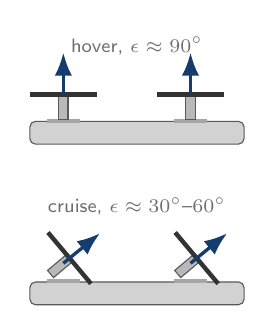
\begin{tikzpicture}[scale=0.85]
      \node[font=\scriptsize, muted] at (0,1.3) {hover, $\epsilon\approx 90^\circ$};
      \aircraft{90}{0}
      \draw[-{Latex}, accent, line width=1.2pt] (0.8,0.6) -- ++(0,0.6);
      \draw[-{Latex}, accent, line width=1.2pt] (-1.1,0.6) -- ++(0,0.6);
      \begin{scope}[yshift=-2.4cm]
        \node[font=\scriptsize, muted] at (0,1.3) {cruise, $\epsilon\approx 30^\circ$--$60^\circ$};
        \aircraft{40}{0}
        \draw[-{Latex}, accent, line width=1.2pt] (0.8,0.45) -- ++(0.55,0.45);
        \draw[-{Latex}, accent, line width=1.2pt] (-1.1,0.45) -- ++(0.55,0.45);
      \end{scope}
    \end{tikzpicture}
  \end{columns}
\end{frame}

\begin{frame}{Why the take-off segment?}
  \begin{itemize}
    \item It is the \textbf{most power-hungry} part of the mission: the rotors carry the full weight,
          the wing carries nothing.
    \item The aircraft moves through \textbf{very different regimes} in a few seconds:
          ground, vertical climb ($\alpha \approx -90^\circ$), partial transition, hover.
    \item Actuators work \textbf{close to their limits} (rotor speed, motor spin-up, tilt rate):
          a heuristic schedule either wastes energy or violates something.
    \item It must end in a state the next segment can start from:
          \textbf{trimmed hover} at the target altitude.
  \end{itemize}
  \vspace{2mm}
  \begin{center}
  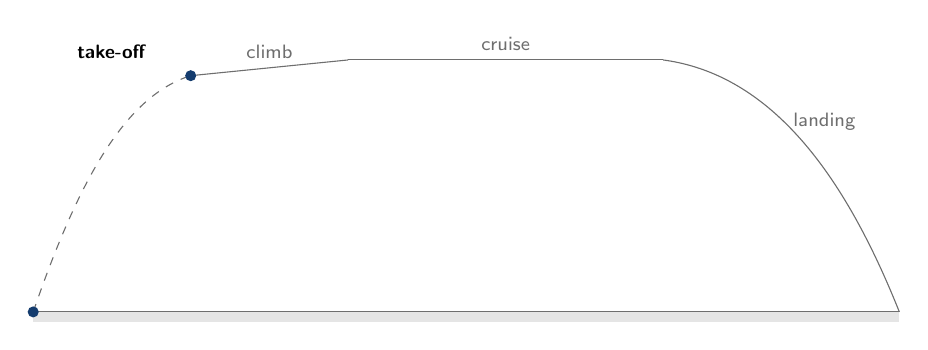
\begin{tikzpicture}[x=1cm,y=0.5cm]
    \draw[muted] (0,0) -- (11,0);
    \fill[gray!20] (0,-0.25) rectangle (11,0);
    \draw[dashed, muted] (0,0) .. controls (0.6,3.5) and (1.2,5.5) .. (2,6);
    \node[font=\scriptsize] at (1.0,6.6) {\textbf{take-off}};
    \draw[muted] (2,6) -- (4,6.4) node[midway, above, font=\scriptsize]{climb};
    \draw[muted] (4,6.4) -- (8,6.4) node[midway, above, font=\scriptsize]{cruise};
    \draw[muted] (8,6.4) .. controls (9.5,6.0) and (10.4,3) .. (11,0) node[pos=0.4, right, font=\scriptsize]{landing};
    \fill[accent] (0,0) circle (2pt) (2,6) circle (2pt);
  \end{tikzpicture}
  \end{center}
\end{frame}

\begin{frame}{Why solve it as an optimisation problem?}
  \begin{columns}[T]
    \column{0.55\textwidth}
    \begin{itemize}
      \item 4 controls, 7 states, one manoeuvre: \textbf{infinitely many} ways to reach 30\,m and hover.
      \item We want the \textbf{best} one for a metric (energy), not just \emph{a} feasible one.
      \item Constraints are part of the problem, not an afterthought:
            rotor limits, actuator rates, attitude, corridor, final trim.
      \item The solver also returns \textbf{sensitivities} (Lagrange multipliers): which limit costs
            how much energy. That is design information.
    \end{itemize}
    \column{0.42\textwidth}
    \centering
    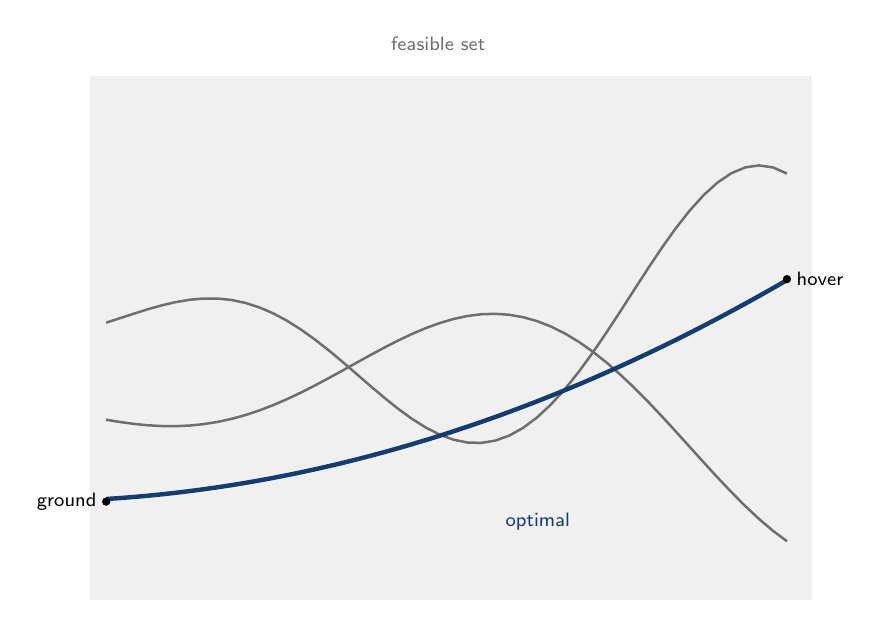
\begin{tikzpicture}
      \begin{axis}[width=\linewidth, height=0.85\linewidth, axis lines=none, xmin=0, xmax=1, ymin=0, ymax=1.05]
        \fill[gray!12] (0.08,0.15) rectangle (0.95,0.95);
        \addplot[muted, line width=0.9pt, domain=0.1:0.92, samples=50] {0.55+0.3*sin(deg(9*x))*x};
        \addplot[muted, line width=0.9pt, domain=0.1:0.92, samples=50] {0.45-0.25*sin(deg(7*x+1))*x};
        \addplot[accent, line width=1.6pt, domain=0.1:0.92, samples=50] {0.3+0.4*x^2};
        \node[font=\scriptsize, accent] at (0.62,0.27) {optimal};
        \node[font=\scriptsize, muted] at (0.5,1.0) {feasible set};
        \fill[black] (0.1,0.3) circle (1.5pt) node[left, font=\scriptsize]{ground};
        \fill[black] (0.92,0.64) circle (1.5pt) node[right, font=\scriptsize]{hover};
      \end{axis}
    \end{tikzpicture}
  \end{columns}
\end{frame}

% =====================================================================
\section{Models}
% =====================================================================

\begin{frame}{Flight dynamics: 3-DOF longitudinal point of view}
  \begin{columns}[T]
    \column{0.47\textwidth}
    \centering
    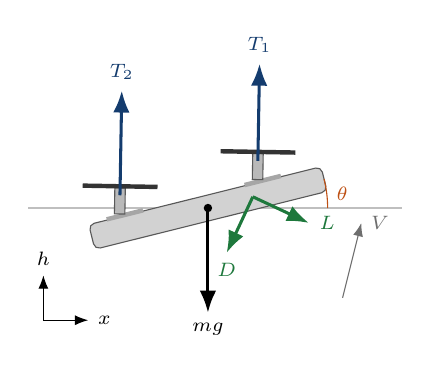
\begin{tikzpicture}[scale=0.95]
      \draw[gray!50] (-2.4,0) -- (2.6,0);
      \aircraft{75}{14}
      \fill (0,0) circle (1.6pt);
      \draw[-{Latex}, black, line width=1.1pt] (0,0) -- (0,-1.4) node[below, font=\scriptsize]{$mg$};
      \draw[-{Latex}, accent, line width=1.1pt] ({0.8*cos(14)-0.45*sin(14)},{0.8*sin(14)+0.45*cos(14)}) -- ++({cos(89)*1.3},{sin(89)*1.3}) node[above, font=\scriptsize]{$T_1$};
      \draw[-{Latex}, accent, line width=1.1pt] ({-1.1*cos(14)-0.45*sin(14)},{-1.1*sin(14)+0.45*cos(14)}) -- ++({cos(89)*1.4},{sin(89)*1.4}) node[above, font=\scriptsize]{$T_2$};
      \draw[-{Latex}, good, line width=1.1pt] (0.6,0.15) -- ++(-0.35,-0.75) node[below, font=\scriptsize]{$D$};
      \draw[-{Latex}, good, line width=1.1pt] (0.6,0.15) -- ++(0.75,-0.35) node[right, font=\scriptsize]{$L$};
      \draw[accent2] (1.6,0) arc (0:14:1.6) node[midway, right, font=\scriptsize]{$\theta$};
      \draw[-{Latex}, muted] (1.8,-1.2) -- ++(0.25,1.0) node[right, font=\scriptsize]{$V$};
      \draw[-{Latex}] (-2.2,-1.5) -- ++(0.6,0) node[right, font=\scriptsize]{$x$};
      \draw[-{Latex}] (-2.2,-1.5) -- ++(0,0.6) node[above, font=\scriptsize]{$h$};
    \end{tikzpicture}
    \column{0.5\textwidth}
    \small
    States $\mathbf{x} = (x, h, v_x, v_h, \theta, q, E)$,\\
    controls $\mathbf{u} = (\epsilon_1, \epsilon_2, n_1, n_2)$.
    \begin{align*}
      \dot x &= v_x, & \dot h &= v_h,\\
      m\,\dot v_x &= F_x, & m\,\dot v_h &= F_h - mg,\\
      \dot\theta &= q, & I_{yy}\,\dot q &= M,\\
      \dot E &= (P_1+P_2)/\eta .
    \end{align*}
    Forces in \textbf{inertial axes}: thrust at $\theta+\epsilon_i$, aero rotated by $\gamma$.
    Well defined in hover, where wind axes are not.
  \end{columns}
\end{frame}

\begin{frame}{Aerodynamics}
  \begin{columns}[T]
    \column{0.5\textwidth}
    \begin{itemize}
      \item Wing, fuselage and tail modelled \textbf{separately}.
      \item $C_L, C_D, C_M$ from tables over the \textbf{full} $\pm 180^\circ$ range,
            smoothed with B-splines: needed because a vertical climb means $\alpha\approx-90^\circ$.
      \item $\bar q = \tfrac12\rho V^2$, $\;L_j = \bar q S_j C_{L,j}(\alpha)$, $\;D_j = \bar q S_j C_{D,j}(\alpha)$.
      \item Regularised airspeed $V = \sqrt{v_x^2+v_h^2+V_\varepsilon^2}$ keeps everything smooth
            when the aircraft is at rest.
    \end{itemize}
    \column{0.47\textwidth}
    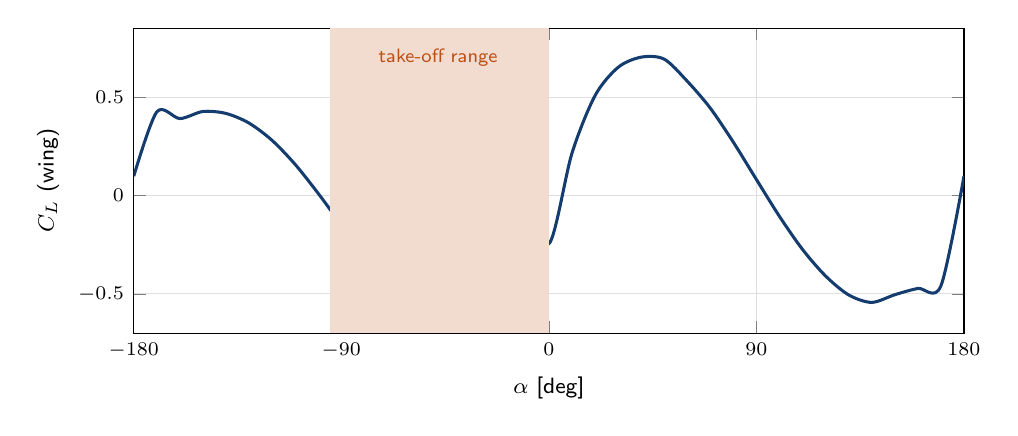
\begin{tikzpicture}
      \begin{axis}[small, xmin=-180, xmax=180, xtick={-180,-90,0,90,180},
                   xlabel={$\alpha$ [deg]}, ylabel={$C_L$ (wing)}, ymin=-0.7, ymax=0.85]
        \addplot[\cA, mark=none, smooth] coordinates {
          (-180,0.0982) (-170,0.425) (-160,0.391) (-150,0.427) (-140,0.417) (-130,0.368) (-120,0.280)
          (-110,0.158) (-100,0.0105) (-90,-0.148) (-80,-0.298) (-70,-0.424) (-60,-0.509) (-50,-0.532)
          (-40,-0.476) (-30,-0.329) (-20,-0.150) (-10,0.0511) (0,-0.245) (10,0.214) (20,0.507)
          (30,0.651) (40,0.703) (50,0.693) (60,0.581) (70,0.444) (80,0.271) (90,0.0814) (100,-0.106)
          (110,-0.274) (120,-0.409) (130,-0.505) (140,-0.543) (150,-0.504) (160,-0.472) (170,-0.459) (180,0.0982)};
        \fill[accent2!20] (axis cs:-95,-0.7) rectangle (axis cs:0,0.85);
        \node[font=\scriptsize, accent2] at (axis cs:-48,0.7) {take-off range};
      \end{axis}
    \end{tikzpicture}
  \end{columns}
\end{frame}

\begin{frame}{Propulsion}
  \begin{columns}[T]
    \column{0.55\textwidth}
    \begin{itemize}
      \item Two rotor groups, $N_e = 2$ rotors each, $D = 0.718$\,m.
      \item Wind-tunnel polynomial fits in advance ratio $J_i = V/(n_i D)$ and inflow angle
            $\phi_i = \alpha + \epsilon_i$:
      \[ T_i = N_e\,C_T(J_i,\phi_i)\,\rho n_i^2 D^4, \qquad P_i = N_e\,C_P(J_i,\phi_i)\,\rho n_i^3 D^5 \]
      \item In-plane force $H_i$ available but currently set to zero.
      \item Rotor speed $n_i$ is a control (no motor dynamics), but its rate is limited.
    \end{itemize}
    \column{0.42\textwidth}
    \centering
    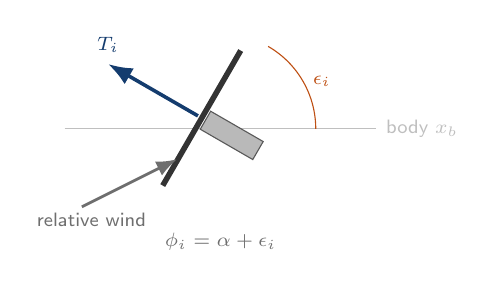
\begin{tikzpicture}[scale=1.1]
      \draw[gray!50] (-1.8,0) -- (1.8,0) node[right, font=\scriptsize]{body $x_b$};
      \begin{scope}[rotate=60]
        \fill[gray!55, draw=gray!70!black] (-0.12,-0.5) rectangle (0.12,0.2);
        \draw[line width=2pt, gray!40!black] (-0.9,0.25) -- (0.9,0.25);
        \draw[-{Latex}, accent, line width=1.3pt] (0,0.3) -- (0,1.5) node[above, font=\scriptsize]{$T_i$};
      \end{scope}
      \draw[accent2] (1.1,0) arc (0:60:1.1) node[pos=0.5, right, font=\scriptsize]{$\epsilon_i$};
      \draw[-{Latex}, muted, line width=1pt] (-1.6,-0.9) -- (-0.5,-0.35) node[pos=0.1, below, font=\scriptsize]{relative wind};
      \node[font=\scriptsize, muted] at (0,-1.3) {$\phi_i = \alpha + \epsilon_i$};
    \end{tikzpicture}
  \end{columns}
\end{frame}

\begin{frame}{Nacelle drag and downwash}
  \begin{columns}[T]
    \column{0.5\textwidth}
    \textbf{Nacelle}: sits in the rotor slipstream, so it sees the induced velocity $v_i$ even in hover.
    Momentum theory, written to stay finite at $V\to0$:
    \[ v_i^4 + 2\sin\phi\,V v_i^3 + V^2 v_i^2 = K^2, \quad K = \frac{T}{\tfrac12\rho D^2} \]
    solved with a few Newton steps from the hover solution $v_i=\sqrt K$, then
    $D_n = C_{D,n}(\alpha_n)\,\tfrac12\rho V_n^2 A_n N_e$.
    \column{0.47\textwidth}
    \textbf{Downwash}: the tail flies in the wing's wake,
    \[ \xi = 0.01 + 0.3\,\alpha, \qquad \alpha_t = \alpha - \xi. \]
    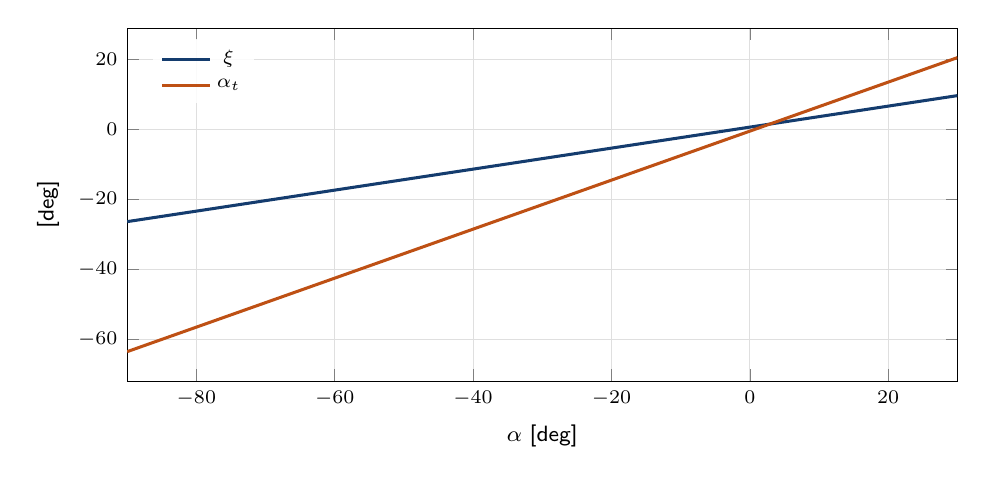
\begin{tikzpicture}
      \begin{axis}[small, height=0.5\linewidth, xmin=-90, xmax=30, xlabel={$\alpha$ [deg]}, ylabel={[deg]},
                   legend pos=north west]
        \addplot[\cA, domain=-90:30] {0.01*180/pi + 0.3*x}; \addlegendentry{$\xi$}
        \addplot[\cB, domain=-90:30] {x - (0.01*180/pi + 0.3*x)}; \addlegendentry{$\alpha_t$}
      \end{axis}
    \end{tikzpicture}
  \end{columns}
\end{frame}

\begin{frame}{Battery}
  \begin{columns}[c]
    \column{0.5\textwidth}
    \begin{itemize}
      \item Kept deliberately simple: an \textbf{energy integrator}.
      \[ \dot E = \frac{P_1 + P_2}{\eta}, \qquad \eta = 0.82 \]
      \item Capacity $E_\text{batt} = 3\,\text{kg}\times 720\,\text{kJ/kg} = 2.16$\,MJ.
      \item The objective is the energy used, as \% of the battery:
            $J = 100\,E(t_f)/E_\text{batt}$.
      \item No voltage, internal resistance or state-of-charge effects yet.
    \end{itemize}
    \column{0.45\textwidth}
    \centering
    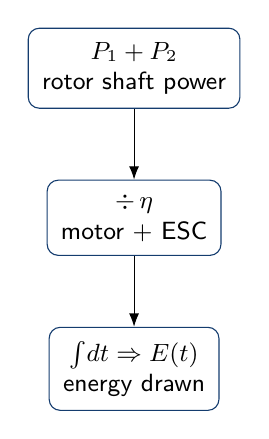
\begin{tikzpicture}[node distance=9mm, every node/.style={font=\small},
        box/.style={draw=accent, rounded corners, inner sep=5pt, align=center}]
      \node[box] (p) {$P_1 + P_2$\\rotor shaft power};
      \node[box, below=of p] (e) {$\div\,\eta$\\motor + ESC};
      \node[box, below=of e] (b) {$\int\! dt \Rightarrow E(t)$\\energy drawn};
      \draw[-{Latex}] (p) -- (e); \draw[-{Latex}] (e) -- (b);
    \end{tikzpicture}
  \end{columns}
\end{frame}

\begin{frame}{Hypotheses}
  \begin{columns}[T]
    \column{0.5\textwidth}
    \begin{itemize}
      \item Rigid body, constant mass ($m = 25.5$\,kg), longitudinal plane only.
      \item Flat, non-rotating Earth; still air, constant density ($\rho = 1.213$\,kg/m$^3$), no ground effect.
      \item Quasi-steady aerodynamics and rotor coefficients.
      \item Both rotors of a group identical; tilt and rotor speed commanded directly.
    \end{itemize}
    \column{0.5\textwidth}
    \begin{itemize}
      \item Rotor--wing interaction only through nacelle drag; no slipstream on the wing.
      \item Elevator not modelled: pitch is controlled by differential thrust and tilt.
      \item Placeholder actuator limits: 50\,rps/s (motors), 45\,$^\circ$/s (tilt servos).
    \end{itemize}
  \end{columns}
\end{frame}

\begin{frame}{Limitations (known and documented)}
  \begin{itemize}
    \item \textbf{Angle of attack} is computed assuming forward body velocity, $u_b \ge 0$:
          backwards flight is forbidden through bounds ($x, v_x \ge 0$).
    \item \textbf{Regularised airspeed} $V_\varepsilon = 0.5$\,m/s: aero forces are slightly non-zero at rest
          (negligible, but present).
    \item \textbf{Fit validity}: propeller fits trusted for $J \le 1.2$, $|\phi| \le 90^\circ$, enforced as constraints.
    \item \textbf{Moment arms}: fuselage and nacelle drag arms inherited from the cruise model are not fully
          consistent; tail moment uses wing reference area. Kept for consistency with cruise, flagged for review.
    \item \textbf{Battery}: energy only, so the optimum cannot see power-dependent losses.
    \item \textbf{Data to confirm}: mass against the CAD, fuselage arms; nacelle drag reuses the fuselage $C_D$ table.
  \end{itemize}
\end{frame}

% =====================================================================
\section{Problem formulation}
% =====================================================================

\begin{frame}{Optimal control problem}
  \begin{center}
  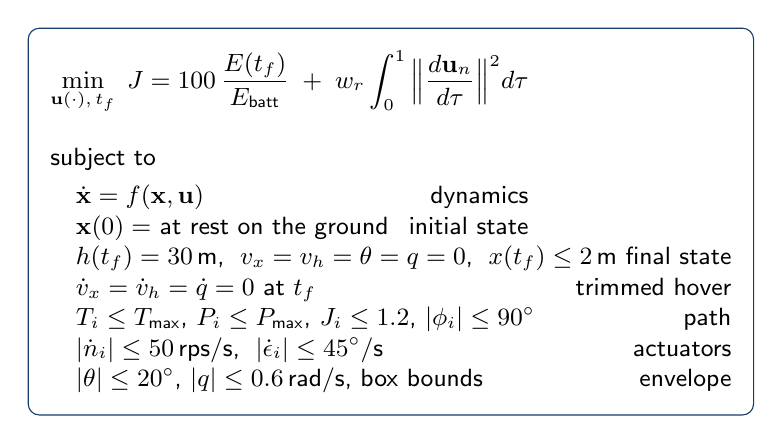
\begin{tikzpicture}
    \node[draw=accent, rounded corners, inner sep=8pt, align=left, font=\small] {%
      $\displaystyle \min_{\mathbf{u}(\cdot),\,t_f}\; J = 100\,\frac{E(t_f)}{E_\text{batt}}
        \;+\; w_r \int_0^1 \Big\|\frac{d\mathbf{u}_n}{d\tau}\Big\|^2 d\tau$\\[4mm]
      subject to\\[1mm]
      \quad $\dot{\mathbf{x}} = f(\mathbf{x},\mathbf{u})$ \hfill dynamics\\
      \quad $\mathbf{x}(0) = $ at rest on the ground \hfill initial state\\
      \quad $h(t_f) = 30$\,m, $\;v_x = v_h = \theta = q = 0$, $\;x(t_f)\le 2$\,m \hfill final state\\
      \quad $\dot v_x = \dot v_h = \dot q = 0$ at $t_f$ \hfill trimmed hover\\
      \quad $T_i \le T_\text{max}$, $P_i \le P_\text{max}$, $J_i \le 1.2$, $|\phi_i| \le 90^\circ$ \hfill path\\
      \quad $|\dot n_i| \le 50$\,rps/s, $\;|\dot\epsilon_i| \le 45^\circ$/s \hfill actuators\\
      \quad $|\theta| \le 20^\circ$, $|q| \le 0.6$\,rad/s, box bounds \hfill envelope};
  \end{tikzpicture}
  \end{center}
  {\small The small regulariser ($w_r = 10^{-3}$, $\approx 0.3\%$ of $J$) removes redundant directions
  between tilt and rotor speed.}
\end{frame}

\begin{frame}{Why a direct method?}
  \begin{columns}[T]
    \column{0.48\textwidth}
    \textbf{Indirect} (Pontryagin)\\[1mm]
    {\small
    \begin{itemize}
      \item Derive costates and optimality conditions by hand.
      \item Path inequality constraints and switching structures must be known in advance.
      \item Tiny convergence region; needs a guess of the costates.
    \end{itemize}}
    \column{0.48\textwidth}
    \textbf{Direct} (discretise, then optimise)\\[1mm]
    {\small
    \begin{itemize}
      \item Turn the problem into a finite NLP and hand it to a solver.
      \item Inequalities, bounds and limits handled naturally.
      \item Guess only states and controls: physically meaningful.
      \item Multipliers still available afterwards $\Rightarrow$ costate estimates for free.
    \end{itemize}}
  \end{columns}
  \vspace{3mm}
  \begin{center}
  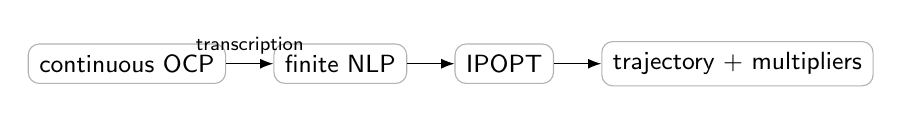
\begin{tikzpicture}[node distance=6mm, every node/.style={font=\small},
      box/.style={draw=gray!60, rounded corners, inner sep=4pt}]
    \node[box] (ocp) {continuous OCP};
    \node[box, right=of ocp] (nlp) {finite NLP};
    \node[box, right=of nlp] (sol) {IPOPT};
    \node[box, right=of sol] (res) {trajectory + multipliers};
    \draw[-{Latex}] (ocp) -- node[above, font=\scriptsize]{transcription} (nlp);
    \draw[-{Latex}] (nlp) -- (sol); \draw[-{Latex}] (sol) -- (res);
  \end{tikzpicture}
  \end{center}
\end{frame}

\begin{frame}{Pipeline}
  \centering
  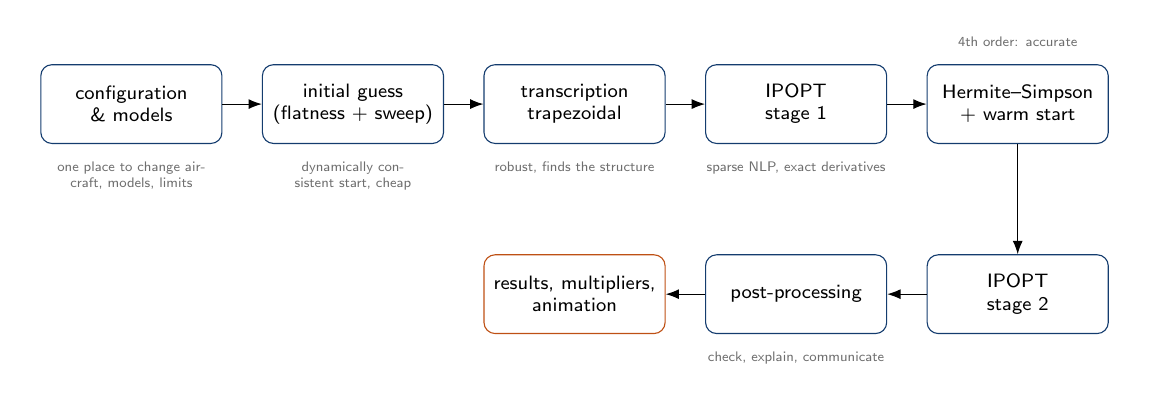
\begin{tikzpicture}[node distance=4mm and 5mm, every node/.style={font=\scriptsize},
      box/.style={draw=accent, rounded corners, inner sep=3pt, align=center, minimum width=2.3cm, minimum height=1cm},
      why/.style={font=\tiny, muted, align=center, text width=2.4cm}]
    \node[box] (cfg) {configuration\\\& models};
    \node[box, right=of cfg] (gue) {initial guess\\(flatness + sweep)};
    \node[box, right=of gue] (tr1) {transcription\\trapezoidal};
    \node[box, right=of tr1] (ip1) {IPOPT\\stage 1};
    \node[box, right=of ip1] (tr2) {Hermite--Simpson\\+ warm start};
    \node[box, below=14mm of tr2] (ip2) {IPOPT\\stage 2};
    \node[box, left=of ip2] (pp) {post-processing};
    \node[box, left=of pp, draw=accent2] (out) {results, multipliers,\\animation};
    \draw[-{Latex}] (cfg) -- (gue); \draw[-{Latex}] (gue) -- (tr1); \draw[-{Latex}] (tr1) -- (ip1);
    \draw[-{Latex}] (ip1) -- (tr2); \draw[-{Latex}] (tr2) -- (ip2); \draw[-{Latex}] (ip2) -- (pp); \draw[-{Latex}] (pp) -- (out);
    \node[why, below=1mm of cfg] {one place to change aircraft, models, limits};
    \node[why, below=1mm of gue] {dynamically consistent start, cheap};
    \node[why, below=1mm of tr1] {robust, finds the structure};
    \node[why, below=1mm of ip1] {sparse NLP, exact derivatives};
    \node[why, above=1mm of tr2] {4th order: accurate};
    \node[why, below=1mm of pp] {check, explain, communicate};
  \end{tikzpicture}
  \par\vspace{3mm}
  {\small Each stage starts from the previous one: the coarse, robust method finds the shape of the
  solution; the accurate one polishes it in a few iterations.}
\end{frame}

\begin{frame}{Transcription: from functions to numbers}
  \begin{columns}[T]
    \column{0.5\textwidth}
    \begin{itemize}
      \item Split $[0,t_f]$ into $N = 40$ intervals; states and controls become values at the nodes.
      \item Dynamics become \textbf{defect} equations the solver must drive to zero:
    \end{itemize}
    {\small
    Trapezoidal (2nd order):
    \[ \mathbf{x}_{k+1} - \mathbf{x}_k - \tfrac{h}{2}(\mathbf{f}_k + \mathbf{f}_{k+1}) = 0 \]
    Hermite--Simpson (4th order):
    \[ \mathbf{x}_{k+1} - \mathbf{x}_k - \tfrac{h}{6}(\mathbf{f}_k + 4\mathbf{f}_m + \mathbf{f}_{k+1}) = 0 \]}
    \vspace{-2mm}
    {\small $t_f$ is a variable: the whole grid stretches with it ($h = t_f/N$).}
    \column{0.47\textwidth}
    \centering
    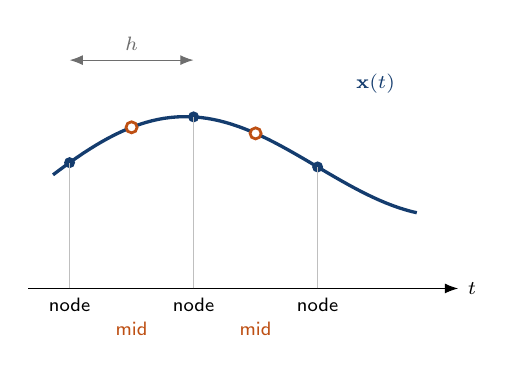
\begin{tikzpicture}[x=1.05cm, y=1cm]
      \draw[-{Latex}] (0,0) -- (5.2,0) node[right, font=\scriptsize]{$t$};
      \draw[accent, line width=1.2pt, domain=0.3:4.7, samples=60] plot (\x, {1.2+0.8*sin(deg(0.9*\x))+0.1*\x});
      \foreach \xx in {0.5,2.0,3.5}{
        \fill[accent] (\xx, {1.2+0.8*sin(deg(0.9*\xx))+0.1*\xx}) circle (2pt);
        \draw[gray!50] (\xx,0) -- (\xx,{1.2+0.8*sin(deg(0.9*\xx))+0.1*\xx});
        \node[below, font=\scriptsize] at (\xx,0) {node};}
      \foreach \xx in {1.25,2.75}{
        \fill[white, draw=accent2, line width=1pt] (\xx, {1.2+0.8*sin(deg(0.9*\xx))+0.1*\xx}) circle (2pt);
        \node[below, font=\scriptsize, accent2] at (\xx,-0.3) {mid};}
      \draw[{Latex}-{Latex}, muted] (0.5,2.9) -- node[above, font=\scriptsize]{$h$} (2.0,2.9);
      \node[font=\scriptsize, accent] at (4.2,2.6) {$\mathbf{x}(t)$};
    \end{tikzpicture}
  \end{columns}
\end{frame}

\begin{frame}{Controls}
  \begin{columns}[T]
    \column{0.55\textwidth}
    \begin{itemize}
      \item $\epsilon_1, \epsilon_2$: tilt of each rotor group. Points the thrust.
      \item $n_1, n_2$: rotor speed of each group. Sets the thrust magnitude.
      \item These are what the aircraft \textbf{actually commands}: servos and motor speed controllers.
      \item 4 controls for 3 equations (2 forces, 1 moment): the problem is \textbf{over-actuated},
            the optimiser chooses how to share the work.
      \item Actuators are rate-limited, so the controls cannot jump between nodes.
    \end{itemize}
    \column{0.42\textwidth}
    \centering
    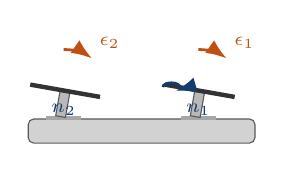
\begin{tikzpicture}[scale=0.9]
      \aircraft{80}{0}
      \draw[-{Latex}, accent2, line width=1pt] (0.8,1.15) arc (90:55:0.7);
      \node[font=\scriptsize, accent2] at (1.45,1.25) {$\epsilon_1$};
      \draw[-{Latex}, accent2, line width=1pt] (-1.1,1.15) arc (90:55:0.7);
      \node[font=\scriptsize, accent2] at (-0.45,1.25) {$\epsilon_2$};
      \draw[accent, line width=1pt, -{Latex}] (0.3,0.62) arc (180:-60:0.12 and 0.06);
      \node[font=\scriptsize, accent] at (0.8,0.3) {$n_1$};
      \node[font=\scriptsize, accent] at (-1.1,0.3) {$n_2$};
    \end{tikzpicture}
  \end{columns}
\end{frame}

\begin{frame}{CasADi and IPOPT}
  \begin{columns}[T]
    \column{0.48\textwidth}
    \textbf{CasADi}: the modelling layer
    {\small
    \begin{itemize}
      \item Symbolic framework with \textbf{automatic differentiation}.
      \item The whole model (aero, rotors, nacelle, moments) is built \emph{once} as an expression graph,
            wrapped in a \texttt{Function} and \emph{mapped} over all nodes.
      \item Exact, sparse Jacobians and Hessians, no finite differences.
      \item \texttt{Opti} stack: variables, constraints and objective written almost as on paper.
    \end{itemize}}
    \column{0.48\textwidth}
    \textbf{IPOPT}: the solver
    {\small
    \begin{itemize}
      \item Interior-point method for large, sparse nonlinear programs.
      \item Handles thousands of variables and constraints and uses the exact Hessian from CasADi.
      \item Inequalities enter through a log-barrier $\mu$, driven to zero.
      \item No need to guess in advance which constraints will be active (unlike active-set SQP).
      \item Open source, robust, standard in trajectory optimisation.
    \end{itemize}}
  \end{columns}
  \vspace{2mm}
  \begin{center}
  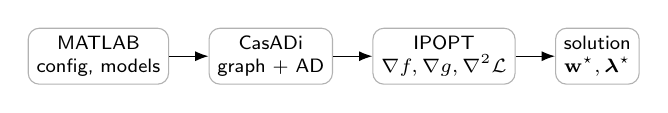
\begin{tikzpicture}[node distance=5mm, every node/.style={font=\scriptsize},
      box/.style={draw=gray!60, rounded corners, inner sep=3pt, align=center}]
    \node[box] (m) {MATLAB\\config, models};
    \node[box, right=of m] (c) {CasADi\\graph + AD};
    \node[box, right=of c] (i) {IPOPT\\$\nabla f, \nabla g, \nabla^2 \mathcal L$};
    \node[box, right=of i] (s) {solution\\$\mathbf{w}^\star, \boldsymbol\lambda^\star$};
    \draw[-{Latex}] (m) -- (c); \draw[-{Latex}] (c) -- (i); \draw[-{Latex}] (i) -- (s);
  \end{tikzpicture}
  \end{center}
\end{frame}

\begin{frame}{The initial guess: differential flatness}
  \begin{columns}[T]
    \column{0.55\textwidth}
    \begin{itemize}
      \item Choose the \textbf{flat outputs} $x(t)$, $h(t)$, $\theta(t)$ as quintic polynomials matching
            position, velocity and acceleration at both ends.
      \item Everything else follows: velocities by differentiation, and the controls by
            \textbf{inverting} the force and moment balance (tilt from the thrust direction,
            rotor speeds from the thrust split that trims the moment).
      \item Built for $t_f \in \{5, 10, 15\}$\,s, checked against bounds, path constraints,
            dynamics and final trim; the best feasible one is kept.
    \end{itemize}
    \column{0.42\textwidth}
    \centering
    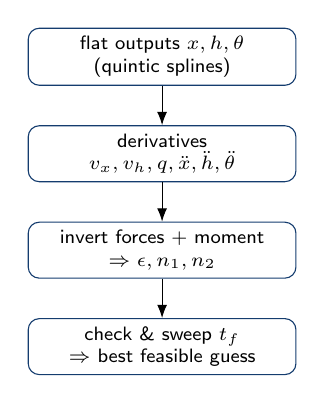
\begin{tikzpicture}[node distance=5mm, every node/.style={font=\scriptsize},
        box/.style={draw=accent, rounded corners, inner sep=3pt, align=center, minimum width=3.4cm}]
      \node[box] (a) {flat outputs $x, h, \theta$\\(quintic splines)};
      \node[box, below=of a] (b) {derivatives\\$v_x, v_h, q, \ddot x, \ddot h, \ddot\theta$};
      \node[box, below=of b] (c) {invert forces + moment\\$\Rightarrow \epsilon, n_1, n_2$};
      \node[box, below=of c] (d) {check \& sweep $t_f$\\$\Rightarrow$ best feasible guess};
      \draw[-{Latex}] (a) -- (b); \draw[-{Latex}] (b) -- (c); \draw[-{Latex}] (c) -- (d);
    \end{tikzpicture}
  \end{columns}
  \vspace{1mm}
  {\small Why: a straight-line guess starts with large defects and often sends IPOPT into restoration; a guess that
  \emph{already obeys the physics} lands it in the right basin and makes runs reproducible.}
\end{frame}

\begin{frame}{What IPOPT actually sees}
  \begin{columns}[T]
    \column{0.52\textwidth}
    \begin{itemize}
      \item One vector of \textbf{nondimensional} unknowns:
            \[ \mathbf{w} = [\,\mathbf{X}_n,\ \mathbf{U}_n,\ \mathbf{U}_{m,n},\ t_f\,] \]
            each state and control divided by its scale, so all are $\mathcal{O}(1)$.
      \item No notion of ``time'' or ``trajectory'': just $f(\mathbf{w})$, $g(\mathbf{w})\le0$, $h(\mathbf{w})=0$.
      \item Scaling + regularisation took the solve from $\sim$600--1200 iterations
            (and different results each run) to $\sim$25--30, reproducibly.
    \end{itemize}
    \column{0.45\textwidth}
    \centering
    {\small
    \begin{tabular}{@{}lrr@{}}
      \toprule
      & trapezoidal & Herm.--Simp. \\
      \midrule
      variables & 452 & 612 \\
      equalities & 295 & 295 \\
      inequalities & 895 & 1215 \\
      \quad of which rates & 320 & 640 \\
      iterations & 28 & 28 \\
      \bottomrule
    \end{tabular}}\\[3mm]
    {\scriptsize\color{muted} plus box bounds on every variable}
  \end{columns}
\end{frame}

\begin{frame}{Lagrange multipliers: the dual variables}
  \begin{columns}[T]
    \column{0.52\textwidth}
    \begin{itemize}
      \item Every constraint $g_j \le 0$ gets a multiplier $\lambda_j \ge 0$.
      \item Meaning: $\lambda_j \approx -\,\partial J^\star/\partial(\text{limit}_j)$,
            the energy saved per unit relaxation of that limit.
      \item Complementarity: either the constraint has slack ($\lambda_j = 0$) or it binds ($\lambda_j > 0$).
            IPOPT ends with $\lambda_j\, s_j \approx \mu \approx 10^{-9}$; the larger factor tells which.
      \item One multiplier \textbf{per node}: they show \emph{when} along the trajectory a limit matters.
            $\sum_k \lambda_k$ is the sensitivity over the whole manoeuvre.
      \item On the defects they are the discrete \textbf{costates} (adjoints).
    \end{itemize}
    \column{0.45\textwidth}
    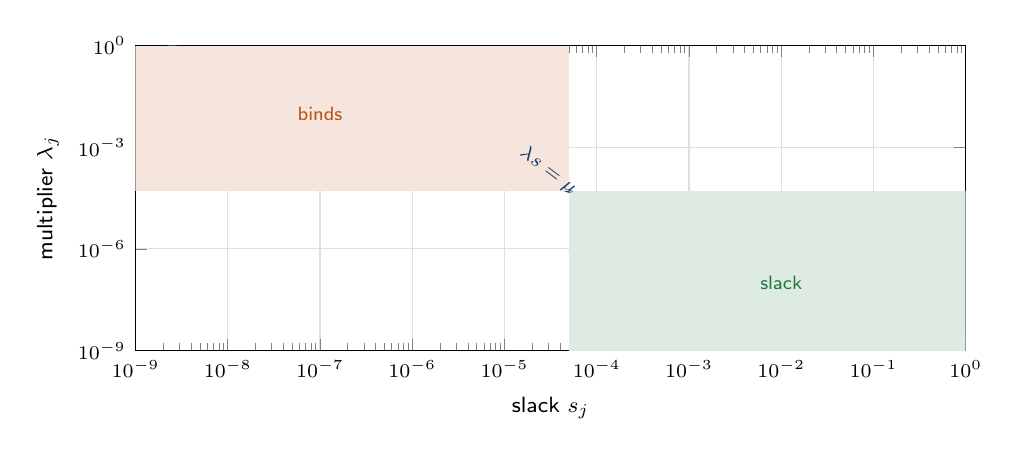
\begin{tikzpicture}
      \begin{axis}[small, xmode=log, ymode=log, xmin=1e-9, xmax=1, ymin=1e-9, ymax=1,
                   xlabel={slack $s_j$}, ylabel={multiplier $\lambda_j$}]
        \addplot[\cA, domain=1e-9:1, samples=40] {2.5e-9/x};
        \fill[accent2!15] (axis cs:1e-9,5e-5) rectangle (axis cs:5e-5,1);
        \fill[good!15] (axis cs:5e-5,1e-9) rectangle (axis cs:1,5e-5);
        \node[font=\scriptsize, accent2] at (axis cs:1e-7,1e-2) {binds};
        \node[font=\scriptsize, good] at (axis cs:1e-2,1e-7) {slack};
        \node[font=\scriptsize, accent, rotate=-37] at (axis cs:3e-5,2e-4) {$\lambda s = \mu$};
      \end{axis}
    \end{tikzpicture}
  \end{columns}
\end{frame}

% =====================================================================
\section{Initial guess}
% =====================================================================

\begin{frame}{Boundary conditions}
  \begin{columns}[c]
    \column{0.5\textwidth}
    {\small
    \begin{tabular}{@{}lll@{}}
      \toprule
      & $t = 0$ & $t = t_f$ \\
      \midrule
      position & $x=0$, $h=0$ & $h = 30$\,m, $x \le 2$\,m \\
      velocity & $0$ & $0$ \\
      attitude & $\theta = q = 0$ & $\theta = q = 0$ \\
      accelerations & -- & $0$ (trimmed) \\
      energy & $E = 0$ & minimise \\
      \bottomrule
    \end{tabular}}
    \column{0.45\textwidth}
    \centering
    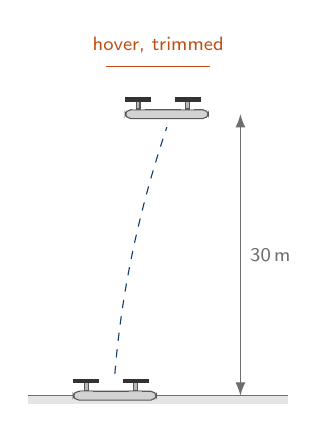
\begin{tikzpicture}[scale=0.55]
      \fill[gray!20] (-2,-0.2) rectangle (4,0);
      \draw[muted] (-2,0) -- (4,0);
      \begin{scope}[scale=0.6] \aircraft{90}{0} \end{scope}
      \draw[dashed, accent] (0,0.5) .. controls (0.2,3) and (0.8,5) .. (1.2,6.2);
      \begin{scope}[shift={(1.2,6.5)}, scale=0.6] \aircraft{90}{0} \end{scope}
      \draw[{Latex}-{Latex}, muted] (2.9,0) -- node[right, font=\scriptsize]{30\,m} (2.9,6.5);
      \draw[accent2] (-0.2,7.6) -- (2.2,7.6);
      \node[font=\scriptsize, accent2] at (1.0,8.1) {hover, trimmed};
    \end{tikzpicture}
  \end{columns}
\end{frame}

\begin{frame}{The selected initial guess}
  \begin{columns}[T]
    \column{0.38\textwidth}
    {\small
    \begin{tabular}{@{}rccc@{}}
      \toprule
      $t_f$ [s] & $J$ [\%] & feasible & \\
      \midrule
      5 & 1.74 & no & $v_h > 10$ \\
      \textbf{10} & \textbf{2.37} & \textbf{yes} & \textbf{selected} \\
      15 & 3.23 & yes & \\
      \bottomrule
    \end{tabular}}\\[3mm]
    {\small A smooth, symmetric climb in 10\,s, rotors near hover speed, tilt $\approx 90^\circ$.
    The 5\,s guess is cheaper but breaks the climb-rate limit.}
    \column{0.6\textwidth}
    \begin{tikzpicture}
      \begin{groupplot}[group style={group size=2 by 2, horizontal sep=1.2cm, vertical sep=0.9cm},
          pres, width=0.52\linewidth, height=0.33\linewidth, xmax=10]
        \nextgroupplot[ylabel={$h$ [m]}]
          \addplot[\cA] table[x=t, y=h]{\tabguess};
        \nextgroupplot[ylabel={$v_h$ [m/s]}]
          \addplot[\cA] table[x=t, y=vh]{\tabguess};
        \nextgroupplot[ylabel={$\epsilon$ [deg]}, xlabel={$t$ [s]}, ymin=85, ymax=95]
          \addplot[\cA] table[x=t, y=eps1]{\tabguess};
        \nextgroupplot[ylabel={$n$ [rps]}, xlabel={$t$ [s]}, ymin=40,
                       legend style={at={(0.5,0.03)}, anchor=south}, legend columns=2]
          \addplot[\cA] table[x=t, y=n1]{\tabguess}; \addlegendentry{$n_1$}
          \addplot[\cB] table[x=t, y=n2]{\tabguess}; \addlegendentry{$n_2$}
      \end{groupplot}
    \end{tikzpicture}
  \end{columns}
\end{frame}

\begin{frame}{What to expect from the optimum}
  \begin{itemize}
    \item The guess is \textbf{feasible but slow}: 10\,s of near-hover costs 2.37\,\% of the battery.
    \item Hovering is expensive, so the optimiser will \textbf{shorten the manoeuvre} and climb as fast as the
          limits allow.
    \item A vertical climb at $\theta = 0$ meets the air flat-on ($\alpha \approx -90^\circ$, maximum drag),
          so expect it to \textbf{pitch up} and tilt the rotors to compensate.
    \item It must still arrive in a trimmed hover, so expect a \textbf{braking phase}
          with the rotors spinning back up at the end, limited by the motors.
  \end{itemize}
\end{frame}

% =====================================================================
\section{Results}
% =====================================================================

\begin{frame}{Headline numbers}
  \begin{columns}[c]
    \column{0.5\textwidth}
    {\small
    \begin{tabular}{@{}lr@{}}
      \toprule
      take-off time & 4.66\,s \\
      energy used & 1.62\,\% of battery \\
      \quad vs.\ initial guess & 2.37\,\% ($-32\%$) \\
      final drift & $x(t_f) = 2.0$\,m \\
      max pitch & $20^\circ$ \\
      max climb rate & 9.4\,m/s \\
      peak power & 11.7\,kW \\
      IPOPT iterations & 28 + 28 \\
      \bottomrule
    \end{tabular}}
    \column{0.45\textwidth}
    \begin{tikzpicture}
      \begin{axis}[pres, height=0.95\linewidth, xmin=0, xmax=2.5, ymin=0, ymax=31, axis equal image=false,
                   xlabel={$x$ [m]}, ylabel={$h$ [m]}]
        \addplot[\cA] table[x=x, y=h]{\tabres};
        \addplot[muted, dashed, line width=0.8pt] coordinates {(2,0) (2,31)};
        \node[font=\scriptsize, muted, rotate=90] at (axis cs:2.15,12) {corridor $x \le 2$\,m};
      \end{axis}
    \end{tikzpicture}
  \end{columns}
\end{frame}

\begin{frame}{Climb and velocities}
  \begin{columns}[T]
    \column{0.5\textwidth}
    \begin{tikzpicture}
      \begin{axis}[pres, xlabel={$t$ [s]}, ylabel={$h$ [m]}, xmax=4.7]
        \addplot[\cA] table[x=t, y=h]{\tabres};
        \addplot[muted, dashed, line width=0.8pt] table[x=t, y=h]{\tabguess};
        \legend{optimum, guess (10\,s)}
      \end{axis}
    \end{tikzpicture}
    \column{0.5\textwidth}
    \begin{tikzpicture}
      \begin{axis}[pres, xlabel={$t$ [s]}, ylabel={[m/s]}, xmax=4.7, legend pos=north east]
        \addplot[\cA] table[x=t, y=vh]{\tabres}; \addlegendentry{$v_h$}
        \addplot[\cB] table[x=t, y=vx]{\tabres}; \addlegendentry{$v_x$}
        \addplot[muted, dashed, line width=0.8pt] coordinates {(0,10) (4.7,10)};
      \end{axis}
    \end{tikzpicture}
  \end{columns}
  {\small Accelerate hard, cruise near the climb-rate limit, then brake into hover: a bang--coast--bang shape
  rounded by the actuator limits. Half the time of the guess.}
\end{frame}

\begin{frame}{Attitude and tilt}
  \begin{columns}[T]
    \column{0.5\textwidth}
    \begin{tikzpicture}
      \begin{axis}[pres, xlabel={$t$ [s]}, ylabel={[deg]}, xmax=4.7, legend pos=south east]
        \addplot[\cA] table[x=t, y=theta]{\tabres}; \addlegendentry{$\theta$}
        \addplot[\cB] table[x=t, y=alpha]{\tabres}; \addlegendentry{$\alpha$}
        \addplot[muted, dashed, line width=0.8pt] coordinates {(0,20) (4.7,20)};
      \end{axis}
    \end{tikzpicture}
    \column{0.5\textwidth}
    \begin{tikzpicture}
      \begin{axis}[pres, xlabel={$t$ [s]}, ylabel={$\epsilon$ [deg]}, xmax=4.7, legend pos=north west]
        \addplot[\cA] table[x=t, y=eps1]{\tabres}; \addlegendentry{$\epsilon_1$ (front)}
        \addplot[\cB] table[x=t, y=eps2]{\tabres}; \addlegendentry{$\epsilon_2$ (rear)}
      \end{axis}
    \end{tikzpicture}
  \end{columns}
  {\small The aircraft pitches up to the $20^\circ$ limit to reduce the flat-plate drag of the climb
  ($\alpha$ from $-83^\circ$ to $-67^\circ$ at peak pitch) and tilts the rotors forward to keep the thrust vertical.}
\end{frame}

\begin{frame}{Rotors: speed, thrust and power}
  \begin{columns}[T]
    \column{0.5\textwidth}
    \begin{tikzpicture}
      \begin{axis}[pres, xlabel={$t$ [s]}, ylabel={$n$ [rps]}, xmax=4.7, ymin=0, ymax=85, legend pos=south west]
        \addplot[\cA] table[x=t, y=n1]{\tabres}; \addlegendentry{$n_1$}
        \addplot[\cB] table[x=t, y=n2]{\tabres}; \addlegendentry{$n_2$}
        \addplot[muted, dashed, line width=0.8pt] coordinates {(0,78.125) (4.7,78.125)};
      \end{axis}
    \end{tikzpicture}
    \column{0.5\textwidth}
    \begin{tikzpicture}
      \begin{axis}[pres, xlabel={$t$ [s]}, ylabel={thrust [N]}, xmax=4.7, legend pos=north east]
        \addplot[\cA] table[x=t, y=T1]{\tabres}; \addlegendentry{$T_1$}
        \addplot[\cB] table[x=t, y=T2]{\tabres}; \addlegendentry{$T_2$}
        \addplot[black] table[x=t, y=Ttot]{\tabres}; \addlegendentry{$T_1+T_2$}
        \addplot[muted, dashed, line width=0.8pt] coordinates {(0,250.5) (4.7,250.5)}; \addlegendentry{$mg$}
      \end{axis}
    \end{tikzpicture}
  \end{columns}
  {\small Front rotors at full speed during lift-off; total thrust drops below the weight to brake the climb
  and returns to exactly $mg$ at the end. $T_1 \ne T_2$ because the arms differ ($T_1 x_w = T_2 x_t$).}
\end{frame}

\begin{frame}{Energy and convergence}
  \begin{columns}[T]
    \column{0.5\textwidth}
    \begin{tikzpicture}
      \begin{axis}[pres, xlabel={$t$ [s]}, ylabel={power [kW]}, xmax=4.7, axis y line*=left]
        \addplot[\cA] table[x=t, y=P]{\tabres};
      \end{axis}
      \begin{axis}[pres, xmax=4.7, axis y line*=right, axis x line=none, ylabel={energy [\% battery]}, grid=none]
        \addplot[\cB] table[x=t, y=E]{\tabres};
      \end{axis}
    \end{tikzpicture}
    \column{0.5\textwidth}
    \begin{tikzpicture}
      \begin{axis}[pres, ymode=log, xlabel={IPOPT iteration}, ylabel={infeasibility}, xmin=0, xmax=28,
                   legend pos=north east, ymin=1e-14, ymax=1e3]
        \addplot[\cA] table[x=k, y=infpr]{\tabconvA}; \addlegendentry{primal, trapezoidal}
        \addplot[\cA, dashed] table[x=k, y=infdu]{\tabconvA}; \addlegendentry{dual, trapezoidal}
        \addplot[\cB] table[x=k, y=infpr]{\tabconvB}; \addlegendentry{primal, H--S}
        \addplot[\cB, dashed] table[x=k, y=infdu]{\tabconvB}; \addlegendentry{dual, H--S}
      \end{axis}
    \end{tikzpicture}
  \end{columns}
  {\small Left: power (blue) and cumulative energy (orange). Right: both stages converge to $10^{-8}$ in under 30 iterations.}
\end{frame}

\begin{frame}{Animation}
  \centering
  % Link opens the video in the system player (path relative to this file).
  % To embed it instead, replace \href by \movie from the 'multimedia' package.
  \href{run:../Images/vtolto_animation.mp4}{%
    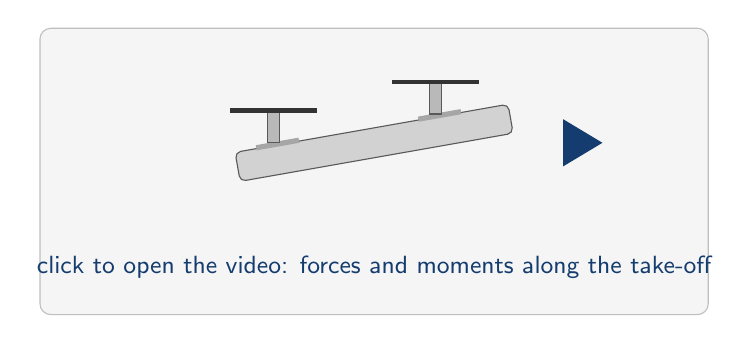
\begin{tikzpicture}
      \draw[gray!50, fill=gray!8, rounded corners] (0,0) rectangle (0.7\textwidth, 0.3\textwidth);
      \begin{scope}[shift={(0.35\textwidth,0.18\textwidth)}, scale=1.1] \aircraft{80}{10} \end{scope}
      \fill[accent] ($(0.35\textwidth,0.18\textwidth)+(2.4,-0.3)$) -- ++(0,0.6) -- ++(0.5,-0.3) -- cycle;
      \node[font=\small, accent] at (0.35\textwidth, 0.05\textwidth) {click to open the video: forces and moments along the take-off};
    \end{tikzpicture}}

  \vspace{2mm}
  {\small Aircraft pitched by $\theta$, rotors tilted by $\epsilon_i$, every force at its point of application,
  moments as arcs, trajectory and time histories alongside.}
\end{frame}

\begin{frame}{Multipliers: where the solution touches a limit}
  \begin{columns}[T]
    \column{0.47\textwidth}
    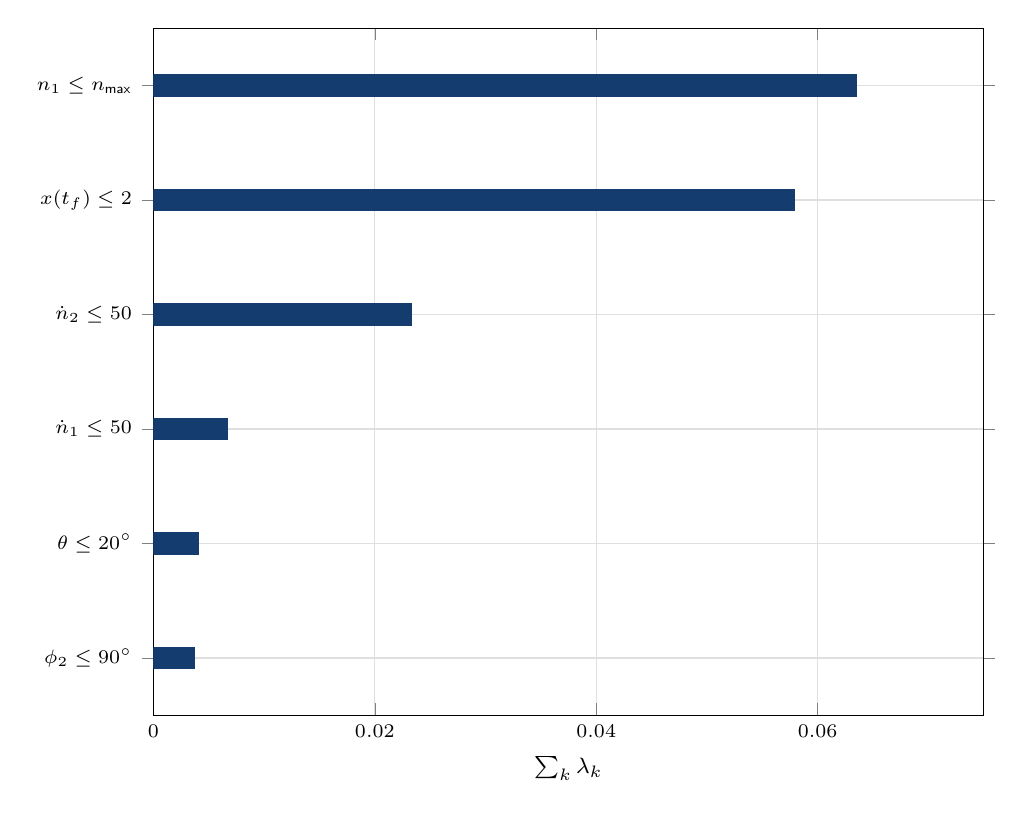
\begin{tikzpicture}
      \begin{axis}[pres, xbar, height=0.85\linewidth, xmin=0, xmax=0.075, enlarge x limits=false,
                   symbolic y coords={phi2,theta,dn1,dn2,xtf,n1}, ytick=data,
                   yticklabels={$\phi_2 \le 90^\circ$, $\theta \le 20^\circ$, $\dot n_1 \le 50$, $\dot n_2 \le 50$, $x(t_f)\le 2$, $n_1 \le n_\text{max}$},
                   xlabel={$\sum_k \lambda_k$}, bar width=7pt, grid=major, xtick={0,0.02,0.04,0.06},
                   scaled x ticks=false, x tick label style={/pgf/number format/fixed}]
        \addplot[fill=accent, draw=accent] coordinates {(0.003615,phi2) (0.003968,theta) (0.006643,dn1) (0.02323,dn2) (0.05782,xtf) (0.06342,n1)};
      \end{axis}
    \end{tikzpicture}
    \column{0.5\textwidth}
    \begin{itemize}\small
      \item[] \textbf{The binding limits are actuators, not aerodynamics.}
      \item \textbf{Rotor speed} at lift-off is the main limit: more rps headroom buys the most energy.
      \item \textbf{Corridor} $x(t_f)\le 2$\,m: pitching up drifts the aircraft forward; it uses all of it.
      \item \textbf{Motor spin-up} before the final hover: the datasheet value matters.
      \item \textbf{Pitch} $\le 20^\circ$ mid-transition; inflow angle only at the very end.
      \item Everything else (thrust, power, $J$, tilt rate) has slack: $\lambda \approx 0$.
    \end{itemize}
  \end{columns}
\end{frame}

\begin{frame}{Multipliers along the trajectory}
  \begin{columns}[T]
    \column{0.5\textwidth}
    \begin{tikzpicture}
      \begin{axis}[pres, xlabel={$t$ [s]}, ylabel={$n_1$ [rps]}, xmax=4.7, axis y line*=left, ymin=0, ymax=85,
                   title={\footnotesize $n_1 \le 78.125$ rps}]
        \addplot[\cA] table[x=t, y=value]{\tablamA};
        \addplot[muted, dashed, line width=0.8pt] coordinates {(0,78.125) (4.7,78.125)};
      \end{axis}
      \begin{axis}[pres, xmax=4.7, axis y line*=right, axis x line=none, ylabel={$\lambda$}, grid=none, ymin=0,
                   scaled y ticks=false, y tick label style={/pgf/number format/fixed}]
        \addplot[ycomb, accent2, line width=1.2pt] table[x=t, y=lam]{\tablamA};
      \end{axis}
    \end{tikzpicture}
    \column{0.5\textwidth}
    \begin{tikzpicture}
      \begin{axis}[pres, xlabel={$t$ [s]}, ylabel={$\dot n_2$ [rps/s]}, xmax=4.7, axis y line*=left, ymin=-60, ymax=60,
                   title={\footnotesize $\dot n_2 \le 50$ rps/s}]
        \addplot[\cA] table[x=t, y=value]{\tablamC};
        \addplot[muted, dashed, line width=0.8pt] coordinates {(0,50) (4.7,50)};
      \end{axis}
      \begin{axis}[pres, xmax=4.7, axis y line*=right, axis x line=none, ylabel={$\lambda$}, grid=none, ymin=0,
                   scaled y ticks=false, y tick label style={/pgf/number format/fixed}]
        \addplot[ycomb, accent2, line width=1.2pt] table[x=t, y=lam]{\tablamC};
      \end{axis}
    \end{tikzpicture}
  \end{columns}
  {\small Blue: the constrained quantity and its limit (dashed). Orange: multiplier at each node. Non-zero only
  where the curve sits on the limit, and its size says how much that instant costs.}
\end{frame}

% =====================================================================
\section{Future work}
% =====================================================================

\begin{frame}{Next: the same problem, convexified}
  \begin{columns}[T]
    \column{0.55\textwidth}
    \textbf{Successive convexification (SCvx)}
    {\small
    \begin{itemize}
      \item Linearise the dynamics around the current trajectory, solve a \textbf{convex} subproblem
            (SOCP) inside a trust region, with virtual controls to keep it feasible; repeat.
      \item Same take-off, solved both ways and compared side by side:
      \begin{itemize}
        \item \textbf{guarantees}: every subproblem is solved to its global optimum, with a certificate (or a proof of infeasibility);
        \item \textbf{runtime}: interior-point on convex cones, predictable and fast;
        \item \textbf{certifiable code}: bounded iterations, embeddable on board;
        \item \textbf{convergence}: proven, under mild assumptions, to a stationary point of the original problem;
        \item \textbf{initial guess}: far less sensitive than nonlinear programming.
      \end{itemize}
    \end{itemize}}
    \column{0.42\textwidth}
    \begin{tikzpicture}
      \begin{axis}[pres, height=0.4\linewidth, axis lines=left, xtick=\empty, ytick=\empty,
                   xlabel={decision}, ylabel={cost}, xmin=0, xmax=4, ymin=0, ymax=3, grid=none,
                   title={\footnotesize nonlinear: many basins}]
        \addplot[\cB, domain=0.1:3.9, samples=80] {1.5+0.6*sin(deg(3*x))+0.08*(x-2)^2};
      \end{axis}
    \end{tikzpicture}\\[1mm]
    \begin{tikzpicture}
      \begin{axis}[pres, height=0.4\linewidth, axis lines=left, xtick=\empty, ytick=\empty,
                   xlabel={decision}, ylabel={cost}, xmin=0, xmax=4, ymin=0, ymax=3, grid=none,
                   title={\footnotesize convex subproblem: one}]
        \addplot[\cA, domain=0.1:3.9, samples=60] {0.4+0.35*(x-2.2)^2};
      \end{axis}
    \end{tikzpicture}
  \end{columns}
\end{frame}

\begin{frame}[plain]
  \centering
  \vfill
  {\Large\color{accent} Thank you}\\[4mm]
  {\small Questions and discussion}\\[8mm]
  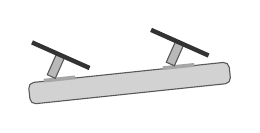
\begin{tikzpicture}[scale=0.8] \aircraft{60}{6} \end{tikzpicture}
  \vfill
\end{frame}

\end{document}
